% Copyright 2004 by Till Tantau <tantau@users.sourceforge.net>.
%
% In principle, this file can be redistributed and/or modified under
% the terms of the GNU Public License, version 2.
%
% However, this file is supposed to be a template to be modified
% for your own needs. For this reason, if you use this file as a
% template and not specifically distribute it as part of a another
% package/program, I grant the extra permission to freely copy and
% modify this file as you see fit and even to delete this copyright
% notice. 

\documentclass[handout]{beamer}
\usepackage{xcolor}
\usepackage[T1]{fontenc}
 \usepackage[flushleft]{threeparttable}
    \usepackage{tabularx}
        \newcolumntype{Z}{>{\centering\arraybackslash}X}
        \newcolumntype{L}{>{\raggedright\arraybackslash}X}
\usepackage{bbm}
\usepackage{dcolumn}
\usepackage{subfig}
        \newcolumntype{d}[1]{D{.}{.}{#1}}

    \usepackage{rotating}               
% There are many different themes available for Beamer. A comprehensive
% list with examples is given here:
% http://deic.uab.es/~iblanes/beamer_gallery/index_by_theme.html
% You can uncomment the themes below if you would like to use a different
% one:
%\usetheme{AnnArbor}
%\usetheme{Antibes}
%\usetheme{Bergen}
%\usetheme{Berkeley}
%\usetheme{Berlin}
%\usetheme{Boadilla}
%\usetheme{boxes}
%\usetheme{CambridgeUS}
%\usetheme{Copenhagen}
%\usetheme{Darmstadt}
%\usetheme{default}
%\usetheme{Frankfurt}
%\usetheme{Goettingen}
%\usetheme{Hannover}
%\usetheme{Ilmenau}
%\usetheme{JuanLesPins}
%\usetheme{Luebeck}
\usepackage{multicol}
\usetheme{Singapore}
\useoutertheme{infolines}
%\usetheme{Malmoe}
%\usetheme{Marburg}
%\usetheme{Montpellier}
%\usetheme{PaloAlto}
%\usetheme{Pittsburgh}
%\usetheme{Rochester}
%\usetheme{Singapore}
%\usetheme{Szeged}
%\usetheme{Warsaw}

\title[Health Inspection]{Does Monitoring Make Food Safer?}

% A subtitle is optional and this may be deleted
\subtitle{}

\author{Jason Huang}
% - Give the names in the same order as the appear in the paper.
% - Use the \inst{?} command only if the authors have different
%   affiliation.

% - Use the \inst command only if there are several affiliations.
% - Keep it simple, no one is interested in your street address.

\date{\today}
% - Either use conference name or its abbreviation.
% - Not really informative to the audience, more for people (including
%   yourself) who are reading the slides online

% This is only inserted into the PDF information catalog. Can be left
% out. 

% If you have a file called "university-logo-filename.xxx", where xxx
% is a graphic format that can be processed by latex or pdflatex,
% resp., then you can add a logo as follows:

% \pgfdeclareimage[height=0.5cm]{university-logo}{university-logo-filename}
% \logo{\pgfuseimage{university-logo}}

% Delete this, if you do not want the table of contents to pop up at
% the beginning of each subsection:


% Let's get started
\begin{document}
\newcommand{\cfbox}[2]{%
    \colorlet{currentcolor}{.}%
    {\color{#1}%
    \fbox{\color{currentcolor}#2}}%
}
\begin{frame}
  \titlepage
\end{frame}



% Section and subsections will appear in the presentation overview
% and table of contents.

\begin{frame}{Motivation}
\begin{itemize}
    \item Sanitation at retail food establishments is a great public health concern but is also difficult for average consumers to enforce or observe
    \pause
    \item Municipal health departments conduct regular food inspections to ensure restaurants uphold hygiene standards
    \begin{itemize}
    \item Dearth of empirical studies that measure the efficacy of inspections on restaurant compliance
    \end{itemize}
    \end{itemize}
    
    \begin{itemize}
    \begin{minipage}{0.7\linewidth}
    \item Major cities, such as New York City, have started to make food inspection results more transparent by having restaurants post grades
    \end{minipage} 
    \begin{minipage}{0.25\linewidth}
    \begin{figure}
    
\includegraphics[scale = 0.1]{grades.jpg}
    \end{figure}
    \end{minipage}
    \begin{itemize}
    \item Inspection results have become more prominent as they become integrated with Yelp
    \end{itemize}
    \end{itemize}
   
\end{frame}

\begin{frame}{Research Questions}
\pause
\begin{itemize}
\item Do inspections incentivize restaurants to improve their sanitation practices?
\begin{itemize}
\item Do restaurants shift attention and effort away from areas that they did well toward areas that got flagged?
\item How do the magnitudes of the results vary across different types of establishments (heterogenous effects)
\end{itemize}
\end{itemize}
\end{frame}

\begin{frame}{Main Findings}
\begin{itemize}
\item Marginal increase in the number of citations leads to improved conditions in subsequent inspections
\begin{itemize}
\item Instead of focusing only on areas that they got cited, restaurants seem to improve in other areas as welll
\end{itemize}
\item More citations also reduces the probability that an establishment receives a complaint call
\end{itemize}
\end{frame}

\begin{frame}{Road Map}
\tableofcontents
\end{frame}
%%%%%%%%%%%%%%%%%%%%%%%%%%%%%%%%%%%%%%%%%%%%%%%%%%
\iffalse
\begin{frame}{Road Map}

\begin{enumerate}
\item Literature Review
\item Background on NYC Food Inspection Program
\item Data 
\item Bunching Around the Thresholds
\item Empirical Analysis
\begin{itemize}
\item Examining the assignments of inspectors
\item Impact of Inspection Results on Subsequent Cleanliness
\item Do harsh inspections hurt restaurant survival?
\end{itemize}
\item Steps Going Forward
\item Discussion and Conclusion
\end{enumerate}
\end{frame}

\section{Literature}
\begin{frame}{1. Literature Review}
Audit and Compliance
\begin{itemize}
\item Restaurants: Jin and Lee (2014, 2016)
\item Environmental Regulation: Duflo et al (2014) 
\item Workplace Safety: Levine, Toffel, and Johnson (2012)
\item Tax: Feinstine (1991), Kleven et al (2011), Gemmell and Ratto (2012)
\end{itemize}
\pause
Specific to NYC Food Inspection System
\begin{itemize}
\item Ho (2012), Meltzer et al (2015), Wong et al (2015)
\end{itemize}
\end{frame}
\fi

%%%%%%%%%%%%%%%%%%%%%%%%%%%%%%%%%%%%%%%%%%%%%%
\section{Background}
\begin{frame}{2. Background on NYC Food Inspection Grading System}
\begin{itemize}
    \pause
    \item Inspection occurs at least once a year
    \begin{itemize}
    \item During inspection, inspector cites violations, assign scores based on severity, and sum up scores
    \end{itemize}
    \pause
    \item Total score is converted to letter grades based on the following cutoffs:
    \begin{itemize}
    \item $\leq$ 13: A
    \item $\geq$ 14 and $\leq 27$: B 
    \item $>$ 28: C
    \end{itemize}
    \pause
    \item Dual Inspection: anything lower than $A$ during initial inspection results in a second inspection within a month
    \begin{itemize}
        \item In the meantime, post previous grade
    \end{itemize}
    \pause
    \item After each inspection, restaurants can pursue adjudication to argue for better grades (in the meantime, post "Grade Pending")
    \begin{itemize}
    \item Resolved within 6 weeks of initial inspection
    \end{itemize}
    \item The health department temporally closes a restaurant if it finds critical violations 
\end{itemize}
\end{frame}

\section{Data}
\subsection{Food Inspection Data}
\begin{frame}{Food Inspection Data}
\begin{itemize}
\item Universe of all food inspections conducted in NYC (2007 - 2016) 
\pause
\item Inspection date and inspector ID
\pause
\item Individual violation codes, total score, corresponding adjudication date, and modified score  
\pause
\item Restaurant level info: name, address, cuisine, service type, and venue type
\end{itemize}
\end{frame}

\subsection{311 Call Data}
\begin{frame}{311 Call Data}
\begin{itemize}
\item 311 is a phone line for non-emergency municipal services - also carries complaint calls to Department of Health and Mental Hygiene concerning restaurants
\begin{itemize}
\item Examples of complaints: 'Rodents/Insects/Garbage', 'Bare Hands in Contact w/ Food', 'Food Contains Foreign Object', 'Food Spoiled', 
\end{itemize}
\item From 2010 to present
\item Each complaint has an incident address and date
\item Use fuzzy string matching on street address to the inspection data
\end{itemize}
\end{frame}

\subsection{Yelp Data}
\begin{frame}{Yelp Data}
\begin{itemize}
\item Acquired start rating and review counts using public API
\item Only the most recent data
\item Successfully matched over 20,000 establishments
\end{itemize}
\end{frame}

\begin{frame}{NYC Food Inspection Pipeline}
\begin{figure}
    \centering
    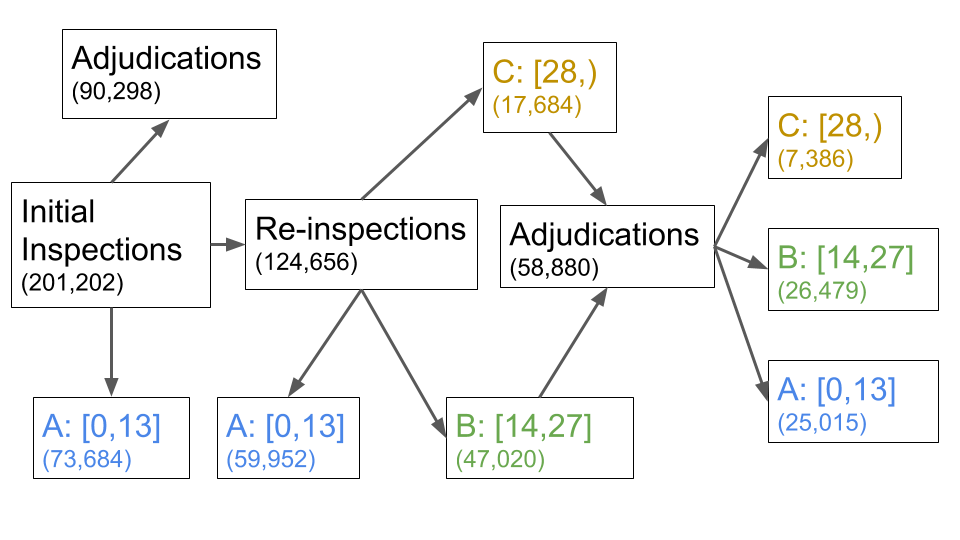
\includegraphics[scale = 0.3]{../../Figures/Scores.png}
    \footnotetext{The numbers in the parenthesis are the number of inspections in those steps}
\end{figure}
\end{frame}
%%%%%%%%%%%%%%%%%%%%%%%%%%%%%%%%%%%%%%%%%%%%%%%%%%%
\iffalse
\begin{frame}{Restaurants are Fully Aware of How Inspections are Scored}
\begin{figure}
    \centering
    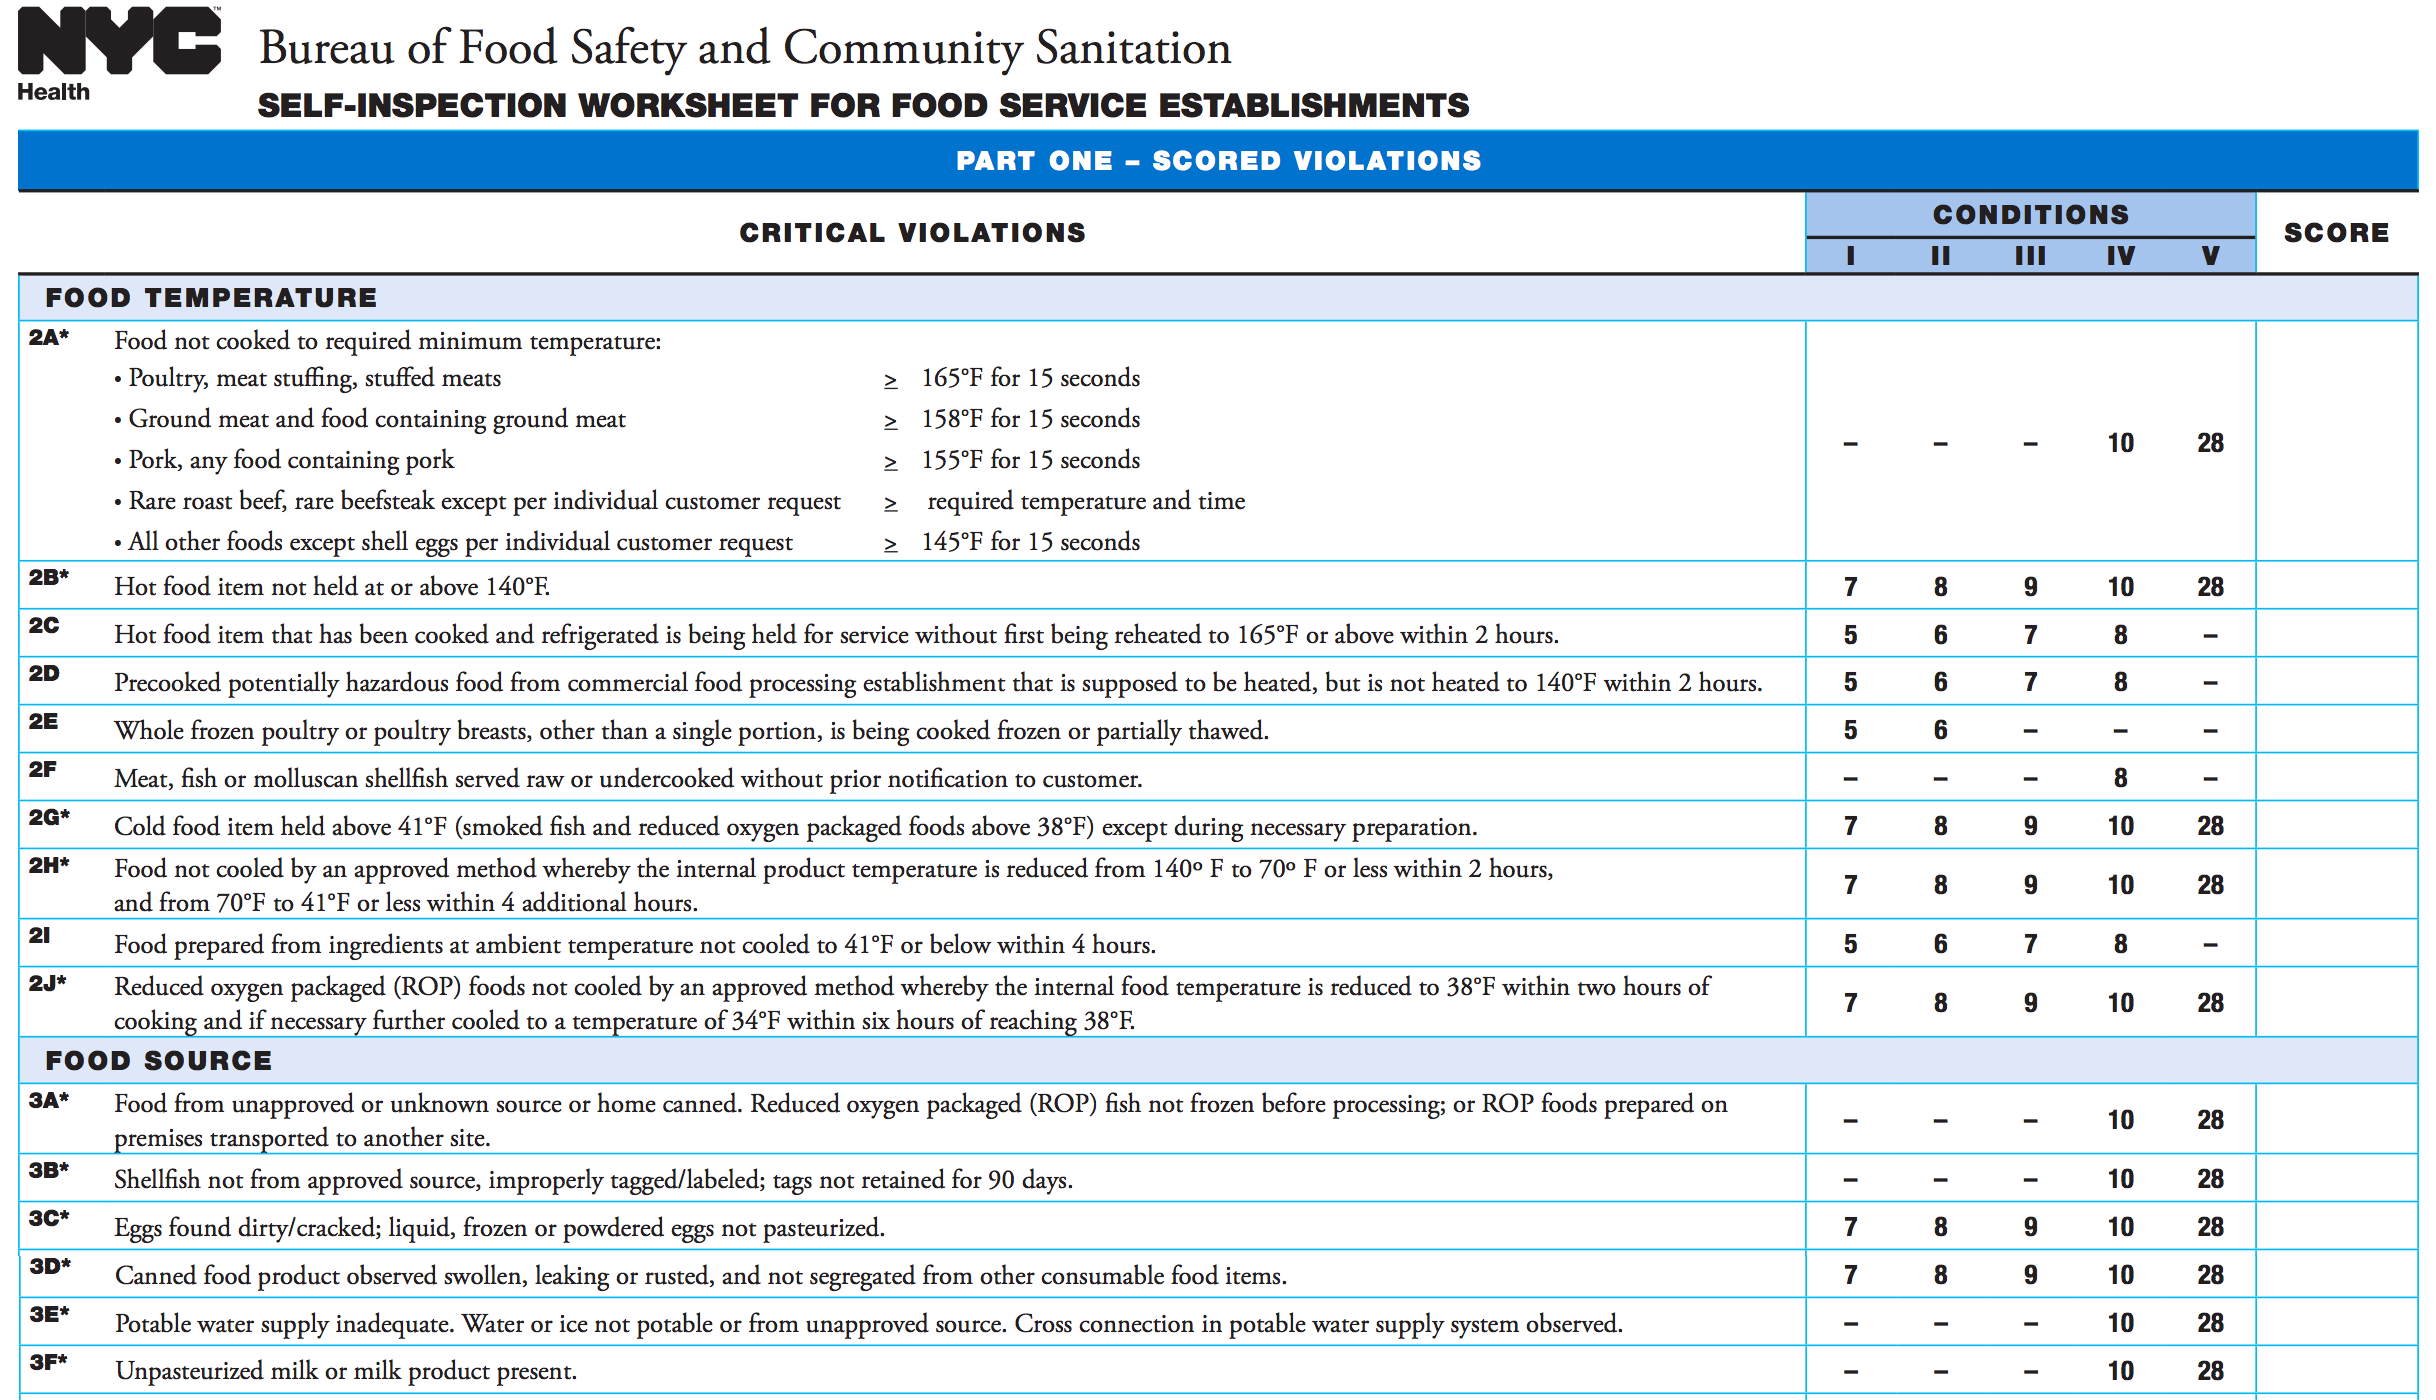
\includegraphics[trim={0 0 0 3cm},clip,scale = 0.28]{self_assessment.png}
\end{figure}
\end{frame}
\begin{frame}{Do More Experienced Restaurants Bunch More?}
\begin{figure}
    \centering
    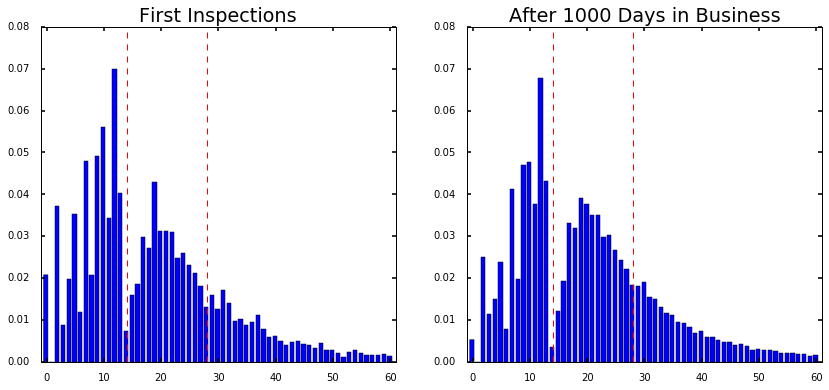
\includegraphics[scale = 0.4]{new_experienced.png}
\end{figure}
Little difference
\end{frame}

\begin{frame}{Do Restaurants Bunch More as They Become More Experienced?}
\begin{itemize}
\item Concern with previous analysis: survivorship bias.
\item Perform local linear weighted regression of probability of getting an A, given that the score is within 2 points of threshold (12 to 15)\footnote{\tiny{Controlling for restaurant FEs and year FEs.}}
\begin{figure}
    \centering
    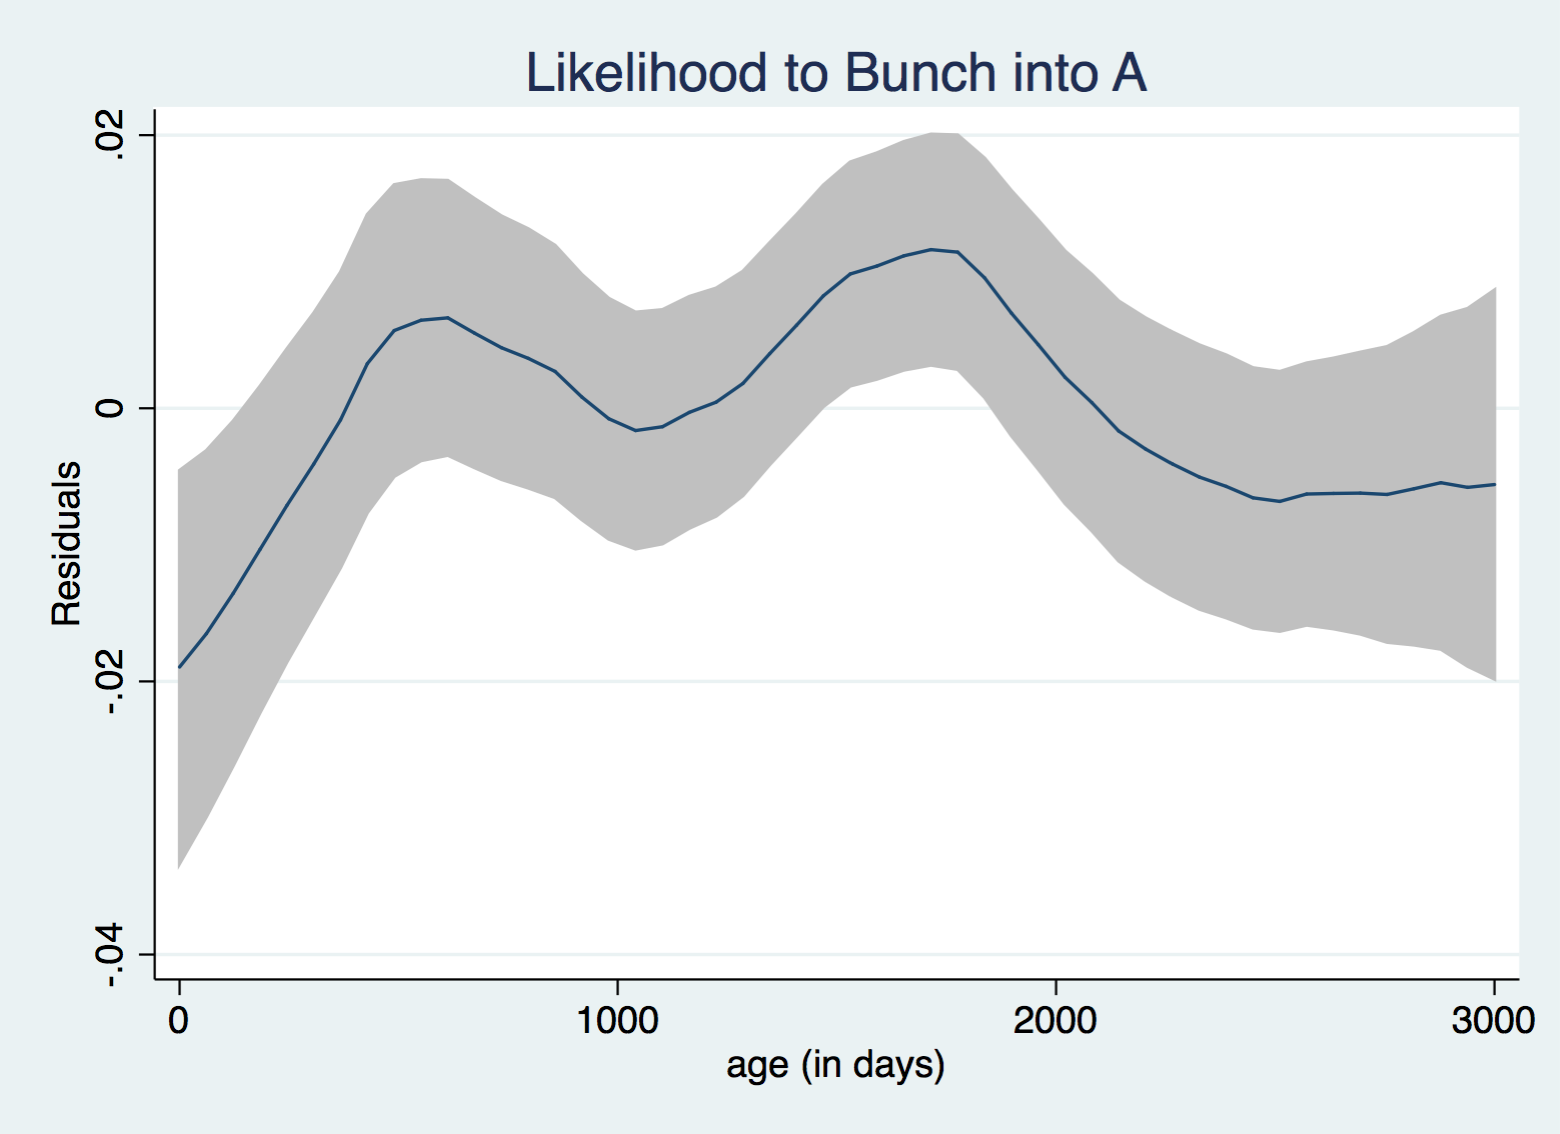
\includegraphics[scale = 0.2]{A_bunch_age.png}
\end{figure}
\item No clear evidence of "learning" through length of time in business
\end{itemize} 
\end{frame}
\fi
%%%%%%%%%%%%%%%%%%%%%%%%%%%%%%%%%%%%%%%%%%%
\section{Impact of Inspections on Restaurant Behaviors}
\begin{frame}{Impact of Inspection Results on Subsequent Inspection Scores}
\pause
    \begin{itemize}
        \item Do inspection results affect sanitation?
        \begin{itemize}
        \pause
        \item Does getting a "bad" score make a restaurant work harder?
        \item Does getting a "good" score cause a restaurant to slack off?
        \end{itemize}
        \pause
        \item Do the inspection results cause restaurants to reallocate efforts across multiple tasks?
    \end{itemize}
    \pause
    Identification strategy: exploit the randomness of inspector assignment and use inspector stringencies as an instrument
\end{frame}

\begin{frame}{Outcomes of Interests from Subsequent Inspections}
\begin{itemize}
\item Overall inspection scores
\item Whether a restaurants receives an A and does not need an re-inspection
\item Whether a restaurant commits critical violations that results in temporarily closure
\end{itemize}
\end{frame}

%%%%%%%%%%%%%%%%%%%%%%%%%%%%%%%%%%%%%%
\iffalse
\begin{frame}{Why should we care about the effects of Scores?}
\begin{itemize}
    \item Indirect monetary reason: scores contribute to letter grades that then can affect business
    \pause
    \item Direct monetary reason: each condition level of each violation is associated with a fine (\$200 - \$1000 after 2014, judges discretion before)
    \pause
    \item Behavior learning reason: restaurants learn about what inspectors are looking for and adjust
\end{itemize}
\end{frame}
\fi
%%%%%%%%%%%%%%%%%%%%%%%%%%%%%%%%%%%%%%%%%%%

\begin{frame}{Empirical Strategy}
    \begin{align*}
        Y_{i,t^{next}} = \beta Score_{i,t} + \delta_i + \tau_{t} + \tau_{t^{next}} + \varepsilon_{it}
    \end{align*}
    \begin{itemize}
    \item $Y_{i,t^{next}}$: outcome from next inspection: overall score, temporary closure, getting an A
    \item $t^{next}$: time period of next inspection
    \item $Score_{i,t^{next}}$: inspection score from the next inspection
    \item $\tau_t$: time fixed effect
    \item $\delta_i$: restaurant fixed effect
    \item $\varepsilon_{it}$: two-way clustered at zipcode and inspector levels\footnote{ (Cameron at el 2009)}
    \end{itemize}
\end{frame}

\begin{frame}{Empirical Strategy}
A challenge of OLS is that $SCORE_{it}$ is endogenous
\begin{itemize}
\item If $\beta$ positive, places that do poorly in the past tend to do poorly in the future
\begin{itemize}
\item Restaurant FE does not fix problem if we have persistence
\end{itemize}
\item If $\beta$ is negative, cannot rule out mechanical mean reversion.  
\end{itemize}
\end{frame}

\subsection{Inspector Specific Stringencies as Instrument}
\begin{frame}{Use Inspector Assignment as Instrument}
Instrument for when inspector $j$ assigned to restaurant $i$
    \begin{align*}
        Z_{ij} = \frac{1}{n_j - I_{ij}} \left( \sum_{kjt\neq ijt}   Y_{kjt}\right)
    \end{align*}
    \begin{itemize}
    \item $n_j$ total number of inspections done by inspector $j$
    \item $I_{ij}$ is the number of times inspector $j$ has inspected restaurant $i$
    \item $Y_{kjt}$ is the outcome used to calculate inspector tendencies
    \end{itemize}
\end{frame}

\begin{frame}{Inspector Stringency is Highly Predictive of Inspection Score}
\begin{align*}
    score_{it} = \gamma Z_{it} + \delta_i + \tau_t + \varepsilon_{it}
\end{align*}
\footnotesize{where $Z_{it}$ is the leave-out propensity of inspector assigned to restaurant $i$ in period $t$.}
\begin{table}[h!]
\centering
\scalebox{0.8}{\begin{tabular}{lccc} \hline
 & (1) & (2) & (3) \\
VARIABLES & Score & Score & Score \\ \hline
 &  &  &  \\
Z & 0.961*** & 0.997*** & 1.135*** \\
 & (0.00948) & (0.00983) & (0.0162) \\
 &  &  &  \\
Observations & 330,469 & 330,466 & 325,681 \\
R-squared & 0.149 & 0.201 & 0.414 \\
Restaurant Controls & NO & YES & NO \\
Restaurant FE & NO & NO & YES \\
 F Statistics & 10271 & 10270 & 4908 \\ \hline
\multicolumn{4}{c}{ Robust standard errors in parentheses} \\
\multicolumn{4}{c}{ *** p$<$0.01, ** p$<$0.05, * p$<$0.1} \\
\end{tabular}
 }
\footnotetext{\tiny{First column consists of all inspections after 10/1/2010. The sample for the second column is reduced to inspections with non-empty zipcode, chain indicator, cuisine type, venue type, and service type. Standard errors are two-way clustered at the inspector and zipcode level.}}
\label{first_stage_reg}
\end{table}
\end{frame}

\begin{frame}{Graphical Representation of First Stage}
    \begin{figure}
        \centering
        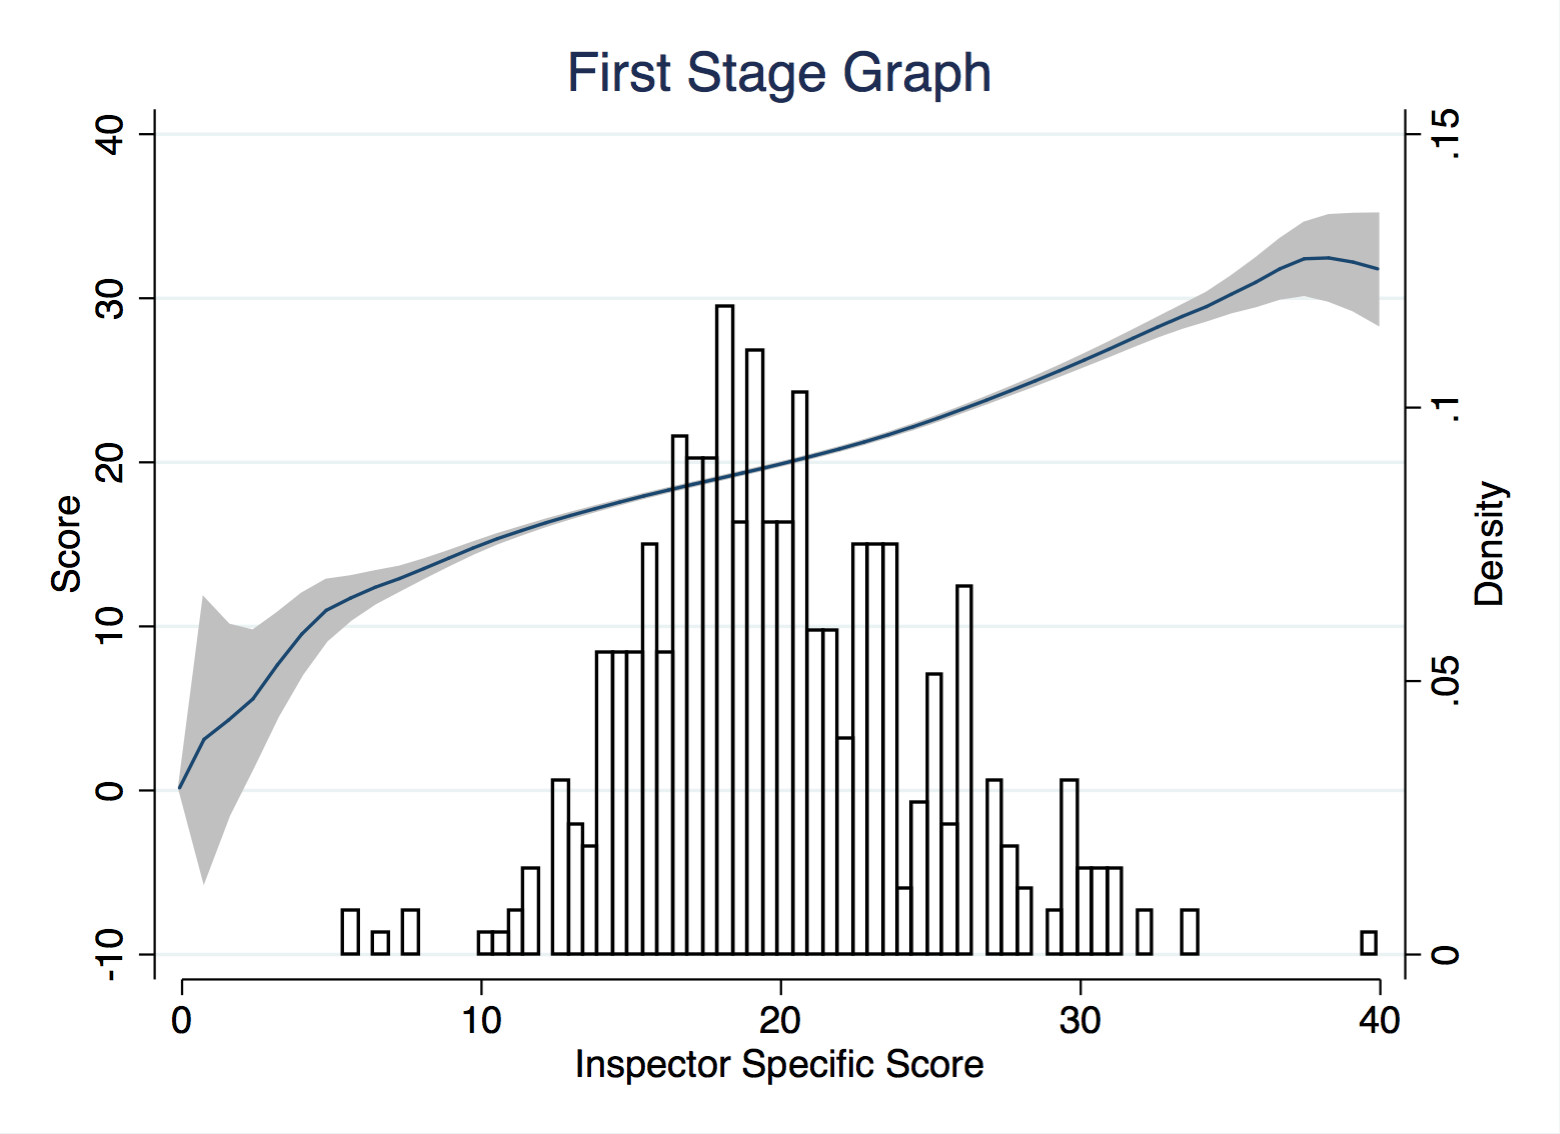
\includegraphics[scale = 0.38]{../../Figures/first_stage_score.png}
    \end{figure}
\end{frame}

\begin{frame}{5. Assignment Process of Inspectors to Restaurants}
\begin{itemize}
\item DOHMH claims that each inspector is randomly assigned to each inspection
\item Implies: 
\begin{align*}
Z_{ijt} = \beta X_i + \delta L_{i,t-1} + \varepsilon,
\end{align*}
with $X_i$ as restaurant characteristics (cuisine, service type, venue type, chain, etc) and $L_{i,t-1}$ as restaurant specific lag terms (previous scores and previous grades), $\beta = \delta = 0$. 

%\tem Inspectors do not specialize based on locations or types of restaurant
%\item The same inspector rarely inspect the same restaurant twice in a roll
%\item An average inspection takes 1.75 hours, and an inspector conducts 3.22 inspections per day. 
\end{itemize}
\end{frame}

\begin{frame}{Coefficients Close to 0 and Insignificant}
\begin{table}
\scalebox{0.5}{
\begin{tabular}{lcccccc} \hline
VARIABLES & Score &  & Inspector Stringency &     & Inspector Stringency  &  \\ 
VARIABLES & (> 50 Inspections) & se &  (> 50 Inspections) & se & (> 650 Inspections) & se \\ \hline
last score & 0.218*** & (0.00746) & -0.000440 & (0.00199) & -0.00193 & (0.00205) \\
last grade = B & 1.430*** & (0.131) & 0.0178 & (0.0628) & 0.0837 & (0.0683) \\
last grade = C & 1.495*** & (0.206) & -0.0494 & (0.0764) & 0.0240 & (0.0807) \\
last inspector propensity & -0.298*** & (0.0104) & -0.00363 & (0.00491) & -0.00529 & (0.00551) \\
chain & -3.644*** & (0.179) & -0.0274 & (0.0644) & -0.0300 & (0.0734) \\
Sea Food & 0.301 & (0.412) & -0.0687 & (0.129) & -0.0648 & (0.136) \\
Chinese & 1.588*** & (0.307) & -0.0952* & (0.0510) & -0.0511 & (0.0546) \\
Pizza/Italian & 0.305** & (0.118) & -0.0893*** & (0.0342) & -0.0614 & (0.0384) \\
Coffee/Tea & -2.219*** & (0.162) & -0.0421 & (0.0889) & -0.0514 & (0.0966) \\
Latin & 1.534*** & (0.303) & -0.0714 & (0.0556) & -0.0390 & (0.0583) \\
Spanish & 1.560*** & (0.261) & 0.0125 & (0.0615) & -0.0435 & (0.0691) \\
Caribbean & 1.542*** & (0.288) & -0.0637 & (0.0608) & -0.0619 & (0.0544) \\
Sandwich & 0.661** & (0.297) & -0.00916 & (0.0472) & 0.0180 & (0.0488) \\
Concession Stands & -4.379*** & (0.722) & 0.295 & (0.197) & 0.209 & (0.211) \\
Fast Food Restaurant-Food Court & 0.570*** & (0.187) & 0.0394 & (0.0881) & -0.0211 & (0.0868) \\
Restaurant  & 1.453*** & (0.158) & 0.0449 & (0.0662) & 0.00343 & (0.0641) \\
Buffet Service & 2.564*** & (0.365) & -0.182* & (0.107) & -0.196 & (0.118) \\
Cater Service & -1.897*** & (0.609) & -0.200 & (0.190) & -0.193 & (0.219) \\
Counter Service & -0.635*** & (0.185) & 0.0273 & (0.0613) & 0.0123 & (0.0684) \\
Take-out Service & -1.410*** & (0.185) & -0.153 & (0.110) & -0.173 & (0.123) \\
Wait Service & 1.205*** & (0.166) & 0.0418 & (0.0481) & 0.0404 & (0.0525) \\
Cafeteria Service & -3.541*** & (0.500) & -0.280* & (0.156) & -0.200 & (0.168) \\
Observations & 299,174 &  & 299,174 &  & 244,099 &  \\
 F Statistics & 101.6 &  & 2.423 &  & 2.249 &  \\ \hline
\multicolumn{7}{c}{ Robust standard errors in parentheses} \\
\multicolumn{7}{c}{ *** p$<$0.01, ** p$<$0.05, * p$<$0.1} \\
\end{tabular}
}
\footnotetext{\tiny{Standard errors are two-way clustered at the inspector and restaurant level.}}
\end{table}
\end{frame}

%%%%%%%%%%%%%%%%%%%%%%%%%%%%%%%%%%%%%%%%%%%%%%%%%%%%%%%%
\iffalse
\begin{frame}{Do inspectors specialize by geography?}
\begin{itemize}
\item Calculate HHIs of Zips that inspectors inspect and HHIs of Inspectors who inspect those Zips
\item Seeing if inspectors focus on certain Zips or certain Zips only get inspected by few inspectors
\end{itemize}
\end{frame}

\begin{frame}
\begin{figure}
    \centering
    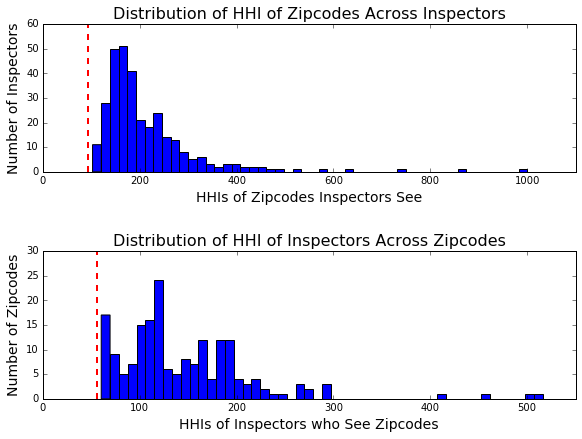
\includegraphics[scale = 0.45]{zip_herf.png}
    \caption{\tiny{HHI for each inspector is based on the distribution of Zipcodes of inspections they conducted. HHI for each zipcode is based on the distribution inspectors that conducted inspections in it.}}
\end{figure}
\end{frame}

\begin{frame}{TSLS Regression Results}
\begin{table}[]
    \centering
\scalebox{0.5}{
\begin{tabular}{lcccc} \hline
\textbf{All Initials Inspections} & (1) & (2) & (3) & (4) \\
VARIABLES & OLS & OLS & IV & IV \\ \hline
 &  &  &  &  \\
Score & 0.182*** & 0.134*** & -0.262*** & -0.233*** \\
 & (0.00763) & (0.00654) & (0.0330) & (0.0253) \\
 &  &  &  &  \\
Observations & 156,323 & 156,317 & 156,323 & 156,317 \\
Restaurant Controls & No & Yes & No & Yes \\
\multicolumn{5}{c}{ Robust standard errors in parentheses} \\
\multicolumn{5}{c}{ *** p$<$0.01, ** p$<$0.05, * p$<$0.1} \\
\end{tabular}
}

\scalebox{0.45}{
\begin{tabular}{lcccc} \hline
\textbf{Initial Scores > 13}  & (1) & (2) & (3) & (4) \\
VARIABLES & OLS & OLS & IV & IV \\ \hline
 &  &  &  &  \\
Score & 0.148*** & 0.115*** & -0.207*** & -0.187*** \\
 & (0.00716) & (0.00650) & (0.0267) & (0.0224) \\
 &  &  &  &  \\
Observations & 104,736 & 104,728 & 104,736 & 104,728 \\
Restaurant Controls & No & Yes & No & Yes \\
\multicolumn{5}{c}{ Robust standard errors in parentheses} \\
\multicolumn{5}{c}{ *** p$<$0.01, ** p$<$0.05, * p$<$0.1} \\
\end{tabular}
}

\scalebox{0.45}{
\begin{tabular}{lcccc} \hline
\textbf{Initial Scores $\leq$ 13}  & (1) & (2) & (3) & (4) \\
VARIABLES & OLS & OLS & IV & IV \\ \hline
 &  &  &  &  \\
Score & 0.613*** & 0.398*** & -3.041*** & -1.902*** \\
 & (0.0229) & (0.0209) & (0.532) & (0.256) \\
 &  &  &  &  \\
Observations & 51,451 & 51,442 & 51,451 & 51,442 \\
Restaurant Controls & No & Yes & No & Yes \\
\multicolumn{5}{c}{ Robust standard errors in parentheses} \\
\multicolumn{5}{c}{ *** p$<$0.01, ** p$<$0.05, * p$<$0.1} \\
\end{tabular}
}
\end{table}
\end{frame}
\fi
%%%%%%%%%%%%%%%%%%%%%%%%%%%%%%%%%%%%%%%%%%%%%%%%%%%%%%%%%%

\subsection{Impact of Violation Citations on Restaurant Cleanliness}
\begin{frame}{TSLS Regression Results}
\begin{table}
\centering
\scalebox{0.6}{\begin{tabular}{lcccccc} \hline
 & (1) & (2) & (3) & (4) & (5) & (6) \\
VARIABLES & Score (OLS) & Score (IV) & Closure (OLS) & Closure (IV) & Grade A (OLS) & Grade A (IV) \\ \hline
 &  &  &  &  &  &  \\
Score & -0.139*** & -0.242*** & -0.000763*** & -0.00101*** & -8.49e-05 & 0.00222*** \\
 & (0.00492) & (0.0162) & (8.26e-05) & (0.000185) & (0.000127) & (0.000556) \\
 &  &  &  &  &  &  \\
Observations & 149,831 & 149,831 & 138,674 & 138,674 & 149,831 & 149,831 \\
Inspection Date FE & YES & YES & YES & YES & YES & YES \\
Restaurant FE & YES & YES & YES & YES & YES & YES \\
 dependent mean & 21.08 & 21.08 & 0.0162 & 0.0162 & 0.372 & 0.372 \\ \hline
\multicolumn{7}{c}{ Robust standard errors in parentheses} \\
\multicolumn{7}{c}{ *** p$<$0.01, ** p$<$0.05, * p$<$0.1} \\
\end{tabular}
}
\footnotetext{\tiny{Standard errors are two-way clustered at zipcode and inspector levels. Closure samples exclude inspections resulting in scores over 28 points.}}
\end{table}
\end{frame}


\subsection{Multi-Tasking}
\begin{frame}{Multi-Dimensionality of Food Inspections}
    \begin{itemize}
    \item Individual Violation Codes Groped into Eight Groups: 
    \begin{figure}
        \centering
        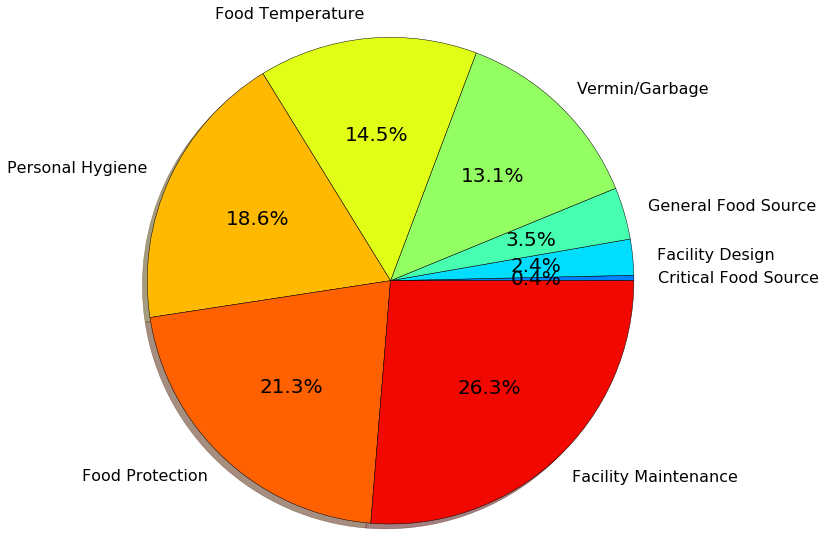
\includegraphics[scale = 0.3]{viol_group_pie.png}
    \end{figure}
    \end{itemize}
\end{frame}

\begin{frame}{Multi-dimensional 1st Stage}
    Instrument Construction:
    \begin{align*}
        Z_{ijg} = \frac{1}{n_j - I_{ij}} \left(\sum_{kjgt \neq ijgt} \# Cited_{ijgt}\right)
    \end{align*}
    \pause
    1st Stage:
    \begin{align*}
        \# Cited_{ijgt} = \sum_{g'\in \mathcal{G}} \theta_{gg'}Z_{ijg'} + \varepsilon_{ijgt} 
    \end{align*}
    \begin{itemize}
    \item $\# Cited_{ijgt}$ is the number of group $g$ violation that inspector $j$ finds in restaurant $i$ at time $t$ and $\mathcal{G}$ is the set of violation groups
    \item $\theta_{gg'}$: measures how inspector's propensity to find violation in group $g'$ relates to one's probability of finding violation in group $g$ 
    \end{itemize}
\end{frame}

\begin{frame}{Multi-task First Stage Equations}
\begin{table}[]
\scalebox{0.4}{
\begin{tabular}{lcccccccc} \hline
 & (1) & (2) & (3) & (4) & (5) & (6) & (7) & (8) \\
VARIABLES & Facility Maintenance & Food Protection & Personal Hygiene & Food Temperature & Vermin/Garbage & Gen. Food Source & Facility Design & Crit. Food Source \\ \hline
 &  &  &  &  &  &  &  &  \\
Facility Maintenance & \textcolor{red}{1.051***} & -0.0550** & 0.0115 & -0.0256* & -0.0104 & 0.00857 & 0.00276 & 0.000821 \\
 & (0.0177) & (0.0227) & (0.0147) & (0.0132) & (0.0139) & (0.00553) & (0.00395) & (0.00139) \\
Food Protection & -0.00719 & \textcolor{red}{0.726***} & -0.00429 & 0.0709* & -0.0911*** & 0.00237 & -0.0105 & 0.00328 \\
 & (0.0372) & (0.0419) & (0.0287) & (0.0388) & (0.0284) & (0.0126) & (0.00883) & (0.00391) \\
Personal Hygiene & 0.00395 & -0.127*** & \textcolor{red}{0.952***} & -0.00446 & -0.0686*** & 0.00179 & -0.00719* & -0.00161 \\
 & (0.0197) & (0.0199) & (0.0192) & (0.0193) & (0.0128) & (0.00524) & (0.00415) & (0.00185) \\
Food Temperature & 0.000328 & -0.0810*** & -0.0890*** & \textcolor{red}{0.808***} & -0.0638*** & 0.00215 & -0.0150** & -0.00488*** \\
 & (0.0236) & (0.0297) & (0.0179) & (0.0226) & (0.0182) & (0.00836) & (0.00609) & (0.00181) \\
Vermin/Garbage & 0.0116 & 0.121** & -0.118*** & -0.186*** & \textcolor{red}{1.011***} & -0.0250 & -0.0274** & -0.00804* \\
 & (0.0486) & (0.0562) & (0.0419) & (0.0601) & (0.0383) & (0.0178) & (0.0136) & (0.00466) \\
Gen. Food Source & -0.00784 & -0.0505 & -0.0105 & -0.0591 & -0.0410 & \textcolor{red}{0.959***} & -0.0233* & 0.00318 \\
 & (0.0456) & (0.0451) & (0.0393) & (0.0407) & (0.0281) & (0.0220) & (0.0129) & (0.00365) \\
Facility Design & -0.0288 & -0.112 & -0.0860 & 0.0153 & -0.116* & -0.0878** & \textcolor{red}{0.845***} & -0.0102 \\
 & (0.0915) & (0.130) & (0.0950) & (0.0930) & (0.0680) & (0.0347) & (0.0256) & (0.0105) \\
Crit. Food Source & -0.0660 & 0.0496 & -0.487* & -0.115 & 0.145 & -0.0241 & -0.0630 & \textcolor{red}{0.921***} \\
 & (0.333) & (0.440) & (0.260) & (0.329) & (0.244) & (0.0868) & (0.0686) & (0.0454) \\
 &  &  &  &  &  &  &  &  \\
Observations & 149,831 & 149,831 & 149,831 & 149,831 & 149,831 & 149,831 & 149,831 & 149,831 \\
 dependent mean & 1.013 & 0.840 & 0.863 & 0.671 & 0.518 & 0.135 & 0.0827 & 0.0149 \\ \hline
\multicolumn{9}{c}{ Robust standard errors in parentheses} \\
\multicolumn{9}{c}{ *** p$<$0.01, ** p$<$0.05, * p$<$0.1} \\
\end{tabular}
}
\end{table}
\end{frame}

\begin{frame}{Multi-dimensional 2nd Stage}
\begin{align*}
    \# Cited_{igt^{next}} = \sum_{g' \in \mathcal{G}} \beta_{gg'} \# Cited_{igt} + \delta_i + \tau_t + \varepsilon_{igt},
\end{align*}
where 
\begin{itemize}
\item $\# Cited_{igt}$: number of group $g$ violations that restaurant $i$ receives on date $t$
\item $\tau_t$: date fixed effect
\item $\delta_i$: restaurant fixed effect
\end{itemize}
\end{frame}
\begin{frame}{How Current Citations Affect Subsequent Citations}
\begin{table}[]
    \centering
    \scalebox{0.4}{
    \begin{tabular}{lcccccccc} \hline
 & (1) & (2) & (3) & (4) & (5) & (6) & (7) & (8) \\
VARIABLES & Facility Maintenance & Food Protection & Personal Hygiene & Food Temperature & Vermin/Garbage & Gen. Food Source & Facility Design & Crit. Food Source \\ \hline
 &  &  &  &  &  &  &  &  \\
Facility Maintenance & \textcolor{red}{-0.236***} & 0.00733 & 0.000184 & -0.00506 & -0.000922 & -0.00159 & 0.000981 & -0.000509 \\
 & (0.00961) & (0.0119) & (0.0107) & (0.00944) & (0.00766) & (0.00380) & (0.00295) & (0.00140) \\
Food Protection & \textcolor{blue}{-0.0776**} & \textcolor{red}{-0.177***} & -0.00731 & -0.0142 & \textcolor{blue}{-0.0397*} & -0.0100 & 0.00372 & \textcolor{brown}{0.00780*} \\
 & (0.0378) & (0.0306) & (0.0410) & (0.0253) & (0.0227) & (0.0113) & (0.0108) & (0.00400) \\
Personal Hygiene & 0.0222 & -0.00484 & \textcolor{red}{-0.189***} & -0.00771 & -0.000551 & 0.00458 & 0.00129 & 0.00217 \\
 & (0.0156) & (0.0103) & (0.0148) & (0.00957) & (0.00892) & (0.00489) & (0.00320) & (0.00173) \\
Food Temperature & 0.0148 & -0.0261 & 0.0133 & \textcolor{red}{-0.214***} & -0.00923 & 0.00613 & -0.00622 & -0.00153 \\
 & (0.0216) & (0.0163) & (0.0162) & (0.0134) & (0.0128) & (0.00722) & (0.00573) & (0.00243) \\
Vermin/Garbage & \textcolor{brown}{0.132***} & \textcolor{blue}{-0.0784*} & 0.00134 & 0.0446 & \textcolor{red}{-0.174***} & 0.0128 & -0.0105 & -0.00126 \\
 & (0.0439) & (0.0404) & (0.0544) & (0.0318) & (0.0283) & (0.0159) & (0.0138) & (0.00404) \\
Gen. Food Source & -0.0114 & -0.00139 & -0.0456 & -0.0103 & \textcolor{blue}{-0.0395*} & \textcolor{red}{-0.191***} & -0.0147 & -0.000895 \\
 & (0.0291) & (0.0348) & (0.0374) & (0.0334) & (0.0202) & (0.0199) & (0.00933) & (0.00395) \\
Facility Design & 0.0265 & \textcolor{blue}{-0.195**} & -0.00742 & 0.0168 & -0.0235 & 0.00421 & \textcolor{red}{-0.199***} & \textcolor{brown}{0.0169*} \\
 & (0.0787) & (0.0925) & (0.0776) & (0.0551) & (0.0612) & (0.0296) & (0.0239) & (0.00977) \\
Crit. Food Source & 0.274 & -0.284 & 0.279 & 0.125 & -0.0346 & -0.0233 & -0.0643 & \textcolor{red}{-0.185***} \\
 & (0.248) & (0.207) & (0.244) & (0.195) & (0.142) & (0.0848) & (0.0682) & (0.0298) \\
Observations & 149,831 & 149,829 & 149,831 & 149,829 & 149,829 & 149,831 & 149,829 & 149,831 \\
Dependent mean & 0.989 & 0.802 & 0.842 & 0.645 & 0.503 & 0.125 & 0.0694 & 0.0126 \\ \hline
\multicolumn{9}{c}{ Robust standard errors in parentheses} \\
\multicolumn{9}{c}{ *** p$<$0.01, ** p$<$0.05, * p$<$0.1} \\
\end{tabular}
}
\footnotetext{Standard errors are two-way clustered at zipcode and inspector levels}
\end{table}
\end{frame}

\subsection{Robustness}
\begin{frame}{Concerns of Empirical Strategy}
Exclusion Restriction
\begin{itemize}
\item Inspectors adjust their grading, given the identities of the previous inspectors
\begin{itemize}
\item Unlikely, given geographically dispersed and random assignment, inspectors need to mentally track the tendencies of hundreds of inspectors
\end{itemize}
\item Inspectors affect restaurant outcomes through channels other than the inspections
\item The causal channel of inspection results is through its influence on the subsequent inspectors' behaviors
\end{itemize}
\pause
Monotonicity condition
\begin{itemize}
    \item The inspection score is strictly increasing in inspector stringency
\end{itemize}
\end{frame}

\begin{frame}{Monotonicity Tests}
\begin{itemize}
\item Because inspections are multi-dimensional, monotonicity might not hold
\begin{itemize}
\item Ex. A frozen yogurt establishment may get a better score from a more stringent inspector if that inspector cares only about hot food being kept above a certain temperature
\end{itemize}
\item Two empirical implications:
\begin{itemize}
\item Test 1: Stringent inspectors should be strict for different types of restaurants 
\begin{itemize}
\item Run first stage for various sub-samples (baseline sample)
\end{itemize}
\item Test 2: Inspectors who are strict for one type of restaurants should be strict for other types
\begin{itemize}
\item Recalculate inspector stringency for each sub-sample with inspection results outside of that sub-sample (inverse-sample)
\end{itemize}
\end{itemize}
\end{itemize}
\end{frame}
\begin{frame}{Monotonicity Test Results}
\begin{table}[h!]
\scalebox{0.45}{\begin{tabular}{lcccc}
\multicolumn{5}{c}{Baseline-Sample} \\ \hline
 & (1) & (2) & (3) & (4) \\
VARIABLES & 1st Quartile & 2nd Quartile & 3nd Quartile & 4th Quartile \\ \hline
Estimate & 0.407*** & 0.681*** & 0.852*** & 1.231*** \\
 & (0.0270) & (0.0240) & (0.0213) & (0.0256) \\
 Observations & 80,172 & 81,817 & 81,901 & 86,433 \\ \hline
\multicolumn{5}{c}{ Robust standard errors in parentheses} \\
\multicolumn{5}{c}{ *** p$<$0.01, ** p$<$0.05, * p$<$0.1} \\
\end{tabular}
 \begin{tabular}{lcccc}
\multicolumn{5}{c}{Inverse-Sample} \\ \hline
 & (1) & (2) & (3) & (4) \\
VARIABLES & 1st Quartile & 2nd Quartile & 3nd Quartile & 4th Quartile \\ \hline
Estimate & 0.369*** & 0.612*** & 0.779*** & 1.609*** \\
 & (0.0340) & (0.0247) & (0.0254) & (0.0674) \\
 Observations & 75,188 & 81,328 & 81,481 & 85,851 \\ \hline
\multicolumn{5}{c}{ Robust standard errors in parentheses} \\
\multicolumn{5}{c}{ *** p$<$0.01, ** p$<$0.05, * p$<$0.1} \\
\end{tabular}
 }

\scalebox{0.45}{\begin{tabular}{lccccc}
\multicolumn{6}{c}{Baseline-Sample} \\ \hline
 & (1) & (2) & (3) & (4) & (5) \\
VARIABLES & Manhattan & Bronx & Brooklyn & Queens & Staten-Isl \\ \hline
Estimate & 1.005*** & 1.082*** & 0.985*** & 0.969*** & 0.944*** \\
 & (0.0156) & (0.0275) & (0.0198) & (0.0206) & (0.0286) \\
 Observations & 131,900 & 31,010 & 79,664 & 77,186 & 10,507 \\ \hline
\multicolumn{6}{c}{ Robust standard errors in parentheses} \\
\multicolumn{6}{c}{ *** p$<$0.01, ** p$<$0.05, * p$<$0.1} \\
\end{tabular}
 \begin{tabular}{lccccc}
\multicolumn{6}{c}{Inverse-Sample} \\ \hline
 & (1) & (2) & (3) & (4) & (5) \\
VARIABLES & Manhattan & Bronx & Brooklyn & Queens & Staten-Is.\\ \hline
Estimate & 0.990*** & 1.082*** & 0.954*** & 0.934*** & 0.938*** \\
 & (0.0269) & (0.0344) & (0.0238) & (0.0248) & (0.0308) \\
 Observations & 128,977 & 30,334 & 76,973 & 74,933 & 10,468 \\ \hline
\multicolumn{6}{c}{ Robust standard errors in parentheses} \\
\multicolumn{6}{c}{ *** p$<$0.01, ** p$<$0.05, * p$<$0.1} \\
\end{tabular}
 }

\scalebox{0.45}{\begin{tabular}{lccccc}
\multicolumn{6}{c}{Baseline-Sample} \\ \hline
 & (1) & (2) & (3) & (4) & (5) \\
VARIABLES & American & Pizza/Italian & Chinese & Coffee & Japanese \\ \hline
Estimate & 0.957*** & 0.994*** & 1.086*** & 0.796*** & 1.096*** \\
 & (0.0241) & (0.0180) & (0.0402) & (0.0354) & (0.0262) \\
 Observations & 75,330 & 38,432 & 38,785 & 13,303 & 10,915 \\ \hline
\multicolumn{6}{c}{ Robust standard errors in parentheses} \\
\multicolumn{6}{c}{ *** p$<$0.01, ** p$<$0.05, * p$<$0.1} \\
\end{tabular}
 \begin{tabular}{lccccc}
\multicolumn{6}{c}{Inverse-Sample} \\ \hline
 & (1) & (2) & (3) & (4) & (5) \\
VARIABLES & American & Pizza/Italian & Chinese & Coffee & Japanese \\ \hline
Estimate & 0.929*** & 0.990*** & 1.070*** & 0.782*** & 1.098*** \\
 & (0.0298) & (0.0199) & (0.0449) & (0.0363) & (0.0273) \\
 Observations & 74,954 & 38,312 & 38,424 & 13,292 & 10,910 \\ \hline
\multicolumn{6}{c}{ Robust standard errors in parentheses} \\
\multicolumn{6}{c}{ *** p$<$0.01, ** p$<$0.05, * p$<$0.1} \\
\end{tabular}
  }

\scalebox{0.45}{\begin{tabular}{lccc}
\multicolumn{4}{c}{Baseline-Sample} \\ \hline
 & (1) & (2) & (3) \\
VARIABLES & Counter Service & Takeout Service & Wait Service \\ \hline
Estimate & 1.055*** & 0.894*** & 1.127*** \\
 & (0.0177) & (0.0140) & (0.0178) \\
 Observations & 127,981 & 127,365 & 73,381 \\ \hline
\multicolumn{4}{c}{ Robust standard errors in parentheses} \\
\multicolumn{4}{c}{ *** p$<$0.01, ** p$<$0.05, * p$<$0.1} \\
\end{tabular}
 \begin{tabular}{lccc}
\multicolumn{4}{c}{Inverse-Sample} \\ \hline
 & (1) & (2) & (3) \\
VARIABLES & Counter Service & Takeout Service & Wait Service \\ \hline
Estimate & 1.064*** & 0.810*** & 1.160*** \\
 & (0.0269) & (0.0181) & (0.0236) \\
 Observations & 126,011 & 124,867 & 72,645 \\ \hline
\multicolumn{4}{c}{ Robust standard errors in parentheses} \\
\multicolumn{4}{c}{ *** p$<$0.01, ** p$<$0.05, * p$<$0.1} \\
\end{tabular}
  }
\footnotetext{\tiny{To reduce noise, only inspections conducted by inspectors who have done at least 50 inspections remain in the regressions.} }
\end{table}
\end{frame}

%%%%%%%%%%%%%%%%%%%%%%%%%%%%
\iffalse
\begin{frame}{More Stringent Inspector More Likely to Cite All Groups}

\begin{align*}
    Pr(Cited_{igt}) = \beta LO\_SCORE_{ij} + \delta X_i + \tau_t \varepsilon
\end{align*}
\begin{table}
\scalebox{0.4}{
\begin{tabular}{lcccccccc} \hline
 & (1) & (2) & (3) & (4) & (5) & (6) & (7) & (8) \\
VARIABLES & Facility Maintenance & Food Protection & Personal Hygiene & Food Temperature & Vermin/Garbage & Gen. Food Source & Facility Design & Crit. Food Source \\ \hline
 &  &  &  &  &  &  &  &  \\
Inspector Propensity & 0.00661*** & 0.0171*** & 0.0162*** & 0.0178*** & 0.0149*** & 0.00477*** & 0.00554*** & 0.00100*** \\
 & (0.00157) & (0.000965) & (0.00111) & (0.00133) & (0.00114) & (0.000753) & (0.000675) & (0.000163) \\
 &  &  &  &  &  &  &  &  \\
Observations & 330,466 & 330,466 & 330,466 & 330,466 & 330,466 & 330,466 & 330,466 & 330,466 \\
 Time FE & YES & YES & YES & YES & YES & YES & YES & YES \\ \hline
\multicolumn{9}{c}{ Robust standard errors in parentheses} \\
\multicolumn{9}{c}{ *** p$<$0.01, ** p$<$0.05, * p$<$0.1} \\
\end{tabular}
}
\end{table}
\end{frame}
\fi
%%%%%%%%%%%%%%%%%%%%%%%%%%%%%%%%%%%%%%%%%%%%%%%%%

\subsection{Complaint Calls}

\begin{frame}{Sample Construction}
\begin{itemize}
\item Convert from inspection level data to a restaurant-month level panel data
\item When an inspection occurs in the middle of a month: 
\begin{itemize}
\item Consider only calls that were made in between the latest event and the end of the month
\item Calculate a weight variable as the fraction of days since the event to the end of the month
\end{itemize}
\end{itemize}
\end{frame}

\begin{frame}{Impact of Restaurant Score on Complaint Call Specification}
\begin{itemize}
\item 2nd Stage
\begin{align*}
    Pr(Called_{it}) = \delta_i + \tau_t + \beta_0 Score_{it} + \beta_1 Month\_Since\_Inspection_{it} \\
    + \beta_2 Month\_Since\_Inspection_{it} \times Score_it + \varepsilon_{it}
\end{align*}
\begin{itemize}
\item $\beta_3$ tests whether the effect of the inspection score changes across time
\end{itemize}
\item Instrument $Score_{it}$ with inspector stringency
\end{itemize}
\end{frame}


\begin{frame}{Results}
\begin{table}
\scalebox{0.5}{\begin{tabular}{lcccccc} \hline
 & (1) & (2) & (3) & (4) & (5) & (6) \\
VARIABLES & Prob Call (OLS) & Prob Call (OLS) & Prob Call (OLS) & Prob Call (IV) & Prob Call (IV) & Prob Call (IV) \\ \hline
 &  &  &  &  &  &  \\
SCORE & -4.68e-05*** & -7.07e-06 & -9.04e-05*** & -8.93e-05* & -9.14e-05* & -6.12e-05 \\
 & (1.54e-05) & (1.57e-05) & (1.79e-05) & (4.76e-05) & (4.98e-05) & (6.16e-05) \\
Months Since Inspection &  & 0.000540*** & -1.94e-05 &  & 0.000498*** & 0.000739* \\
 &  & (3.73e-05) & (6.63e-05) &  & (4.33e-05) & (0.000434) \\
c.mon\_from\_inspect\#c.SCORE &  &  & 5.03e-05*** &  &  & -2.19e-05 \\
 &  &  & (5.81e-06) &  &  & (3.96e-05) \\
 &  &  &  &  &  &  \\
Observations & 1,223,207 & 1,223,207 & 1,223,207 & 1,223,207 & 1,223,207 & 1,223,207 \\
Year-Month FE & YES & YES & YES & YES & YES & YES \\
Restaurant FE & YES & YES & YES & YES & YES & YES \\
 Dependent Mean & 0.0145 & 0.0145 & 0.0145 & 0.0145 & 0.0145 & 0.0145 \\ \hline
\multicolumn{7}{c}{ Robust standard errors in parentheses} \\
\multicolumn{7}{c}{ *** p$<$0.01, ** p$<$0.05, * p$<$0.1} \\
\end{tabular}
}
\end{table}
\end{frame}

%%%%%%%%%%%%%%%%%%%%%%%%%%%%
\iffalse

\begin{frame}
\begin{figure}
\centering
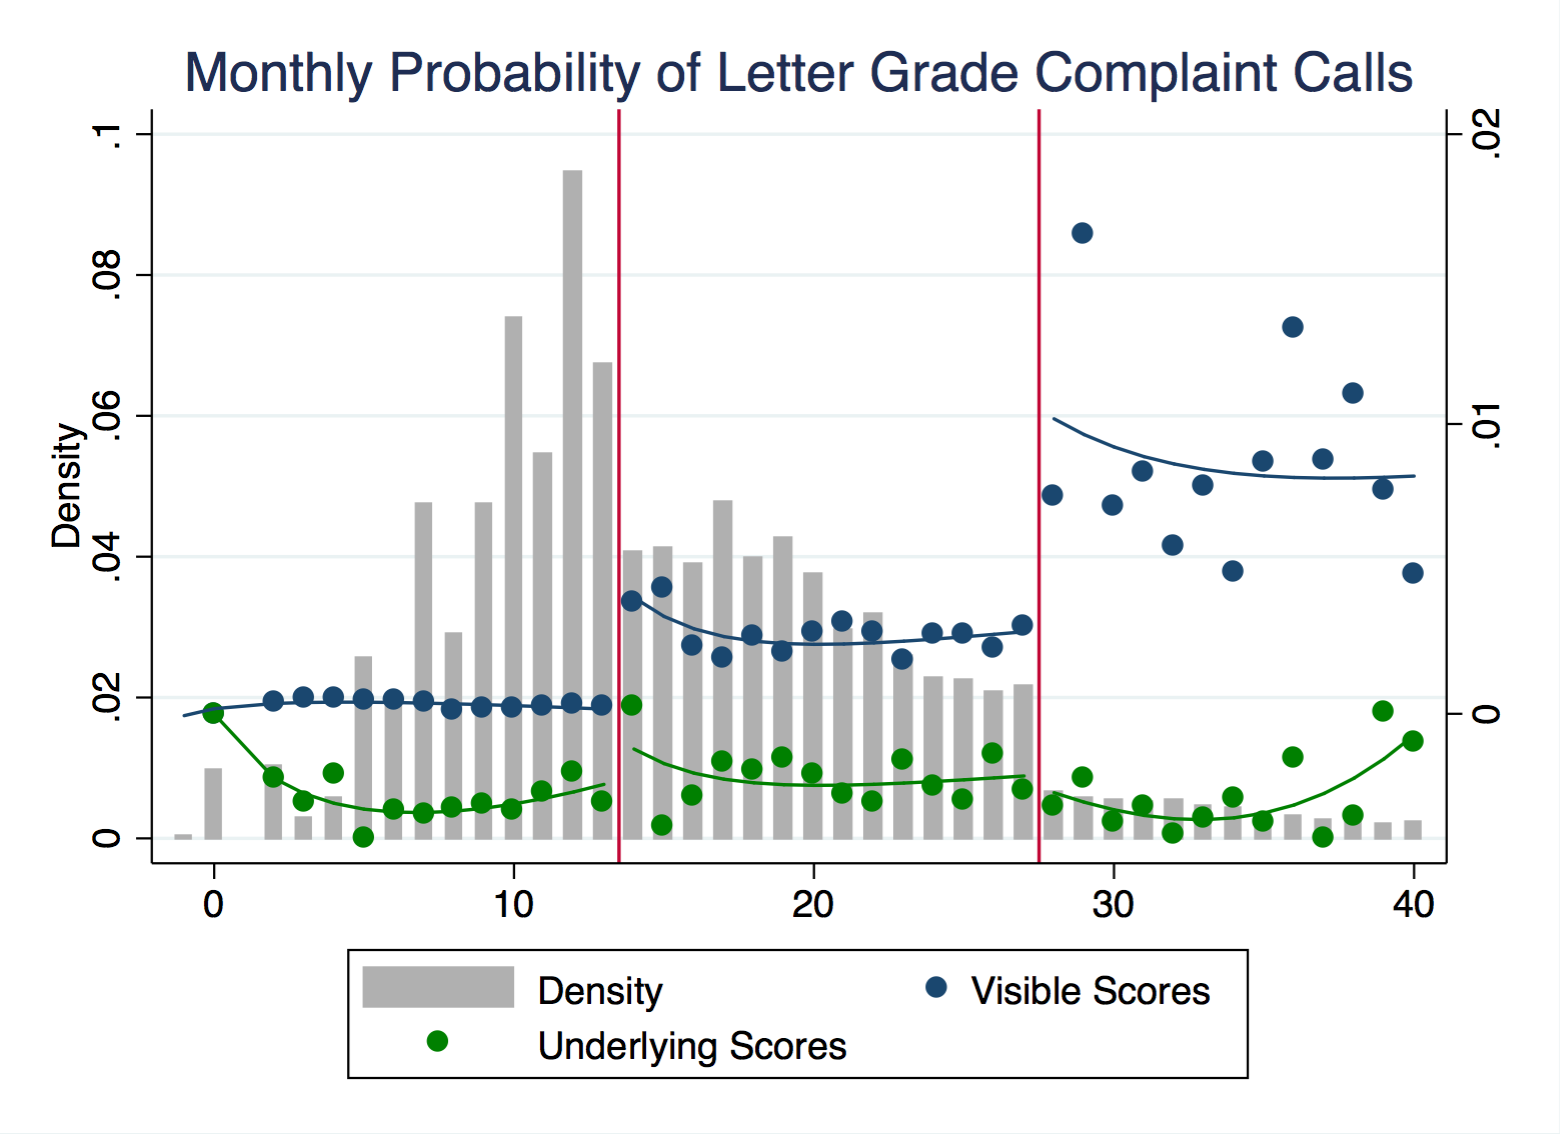
\includegraphics[scale = 0.35]{../../Figures/Calls/score_calls_hist_vis}
\footnotetext{\tiny{The grey density is the histogram of scores after adjudication. Visible scores are ones given post adjudication. Underlying scores are the ones given during cycle-inspections and may not contribute to letter grades.}  }
\end{figure}
\end{frame}

\begin{frame}
\begin{figure}
\centering
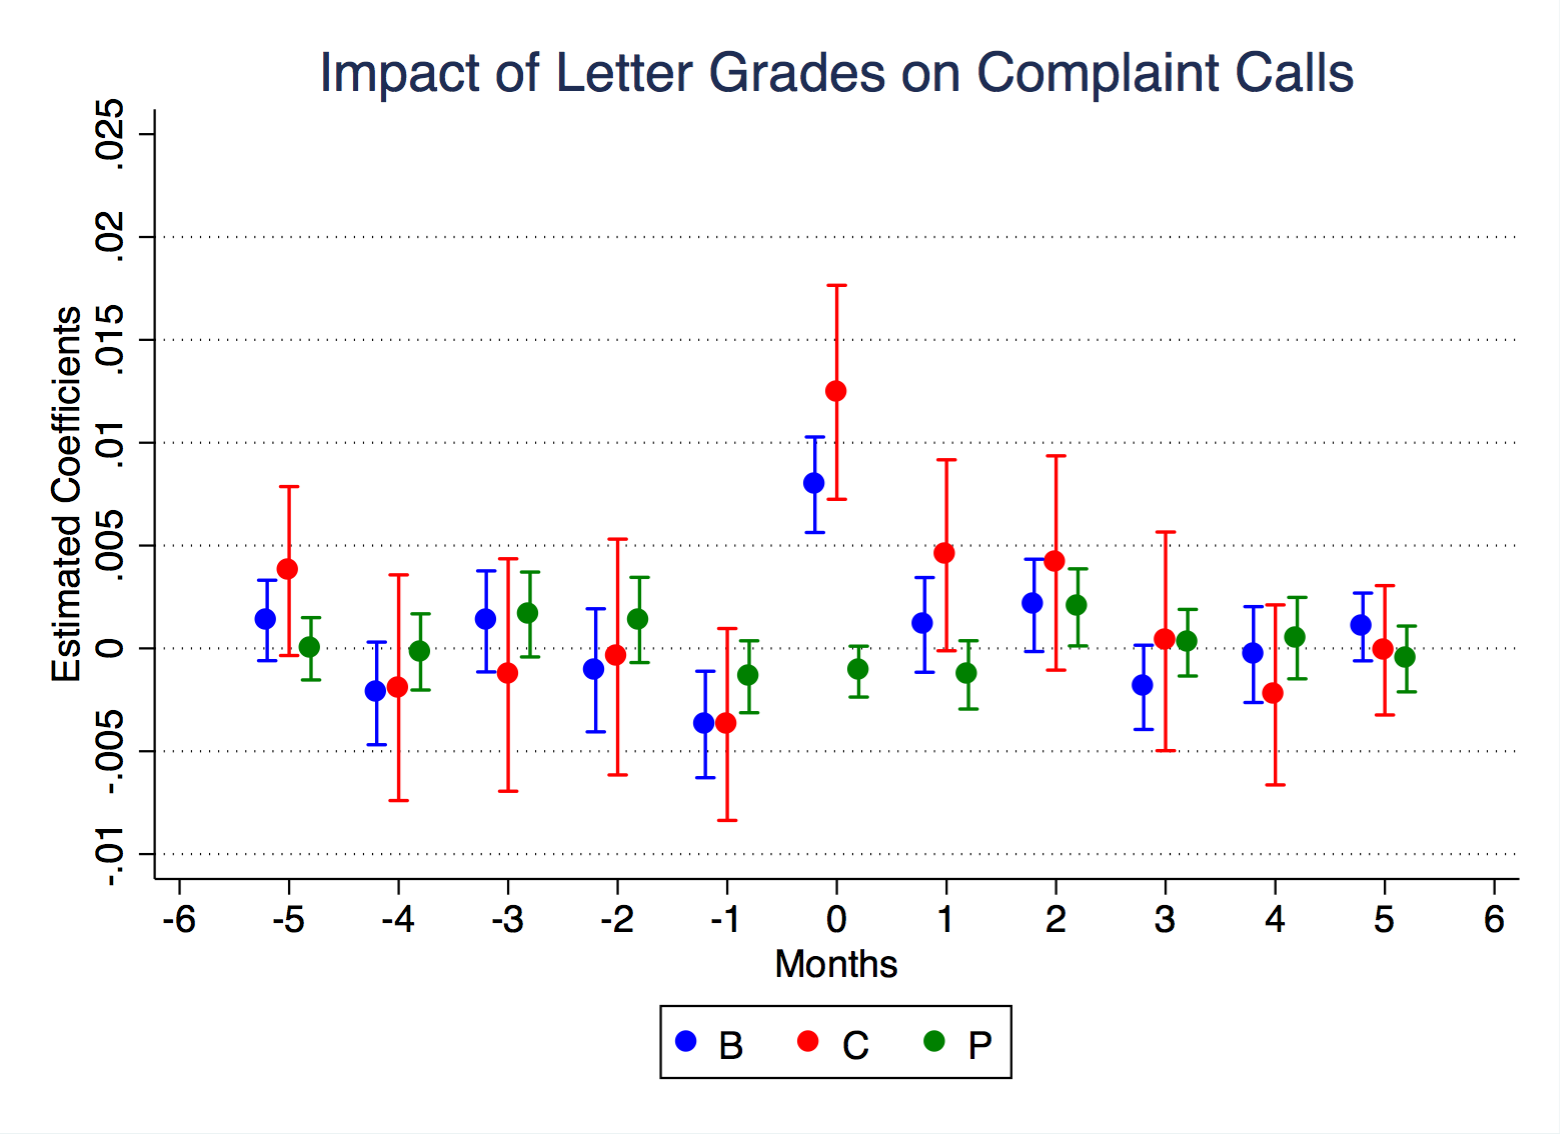
\includegraphics[scale = .35]{../../Figures/Calls/lead_lag_calls_letter}
\footnotetext{\tiny{B, C, and P refers to letter grade B, C, and Grade Pending, respectively. }}
\end{figure}
\end{frame}


\begin{frame}{How does Inspection Grades Affect Restaurant Survivals?}
\begin{itemize}
\item Restaurant industry is high churn, and measuring government regulation hurts these business has policy implication
\item Other studies that use Dif-in-Dif of changes grades suffer from spurious correlation
\item I do not observe exact date of closure
\begin{itemize}
\item Infer based on having no inspections since 2014. 
\item Over counting closures
\item Confirm my counts using Yelp or other data sources
\end{itemize}
\end{itemize}
\end{frame}

\begin{frame}{Empirical Strategy}
\begin{itemize}
\item Convert from inspection level data to a restaurant-year level panel data
\begin{itemize}
\item Restaurants that receive higher scores experience their next inspections earlier, biasing their survival calculations 
\end{itemize}
\item
\begin{align*}
    Pr(Open_{i,t+1}) = \delta_i + \tau_t + SCORE^{avg}_{it} + \varepsilon_{it} \\
    SCORE^{avg}_{it} = \gamma Z^{avg}_{it} + \delta_i + \tau + \epsilon_t
\end{align*}
where $SCORE^{avg}_{it}$ and $Z^{avg}_{it}$ are the average score and inspector propensity seen by restaurant $i$ in year $t$. 
\end{itemize}
\end{frame}

\begin{frame}{Restaurant Survival Summary Statistics}
\begin{table}[htbp]\centering
\caption{\label{year_by_open_next} 
\textbf{Annual Closure Rates}}
\begin{tabular} {@{} l r  r r @{}} \\ \hline
& \multicolumn{3}{@{} c @{}}{\textbf{}} \\
\textbf{} & 
closed &open &Total \\  \hline
2008&     18.6&     81.4&    100.0\\
2009&     18.8&     81.2&    100.0\\
2010&     15.4&     84.6&    100.0\\
2011&     15.7&     84.3&    100.0\\
2012&     15.2&     84.8&    100.0\\
2013&     14.8&     85.2&    100.0\\
2014&     14.5&     85.5&    100.0\\
Total&     16.0&     84.0&    100.0\\\hline 
\multicolumn{4}{@{}l}{}
\end{tabular}
\end{table}
\end{frame}

\begin{frame}{Inspection Results and Restaurant Survival}
\begin{table}[]
    \centering
    \scalebox{0.7}
    {
\begin{tabular}{lcc} \hline
 & (1) & (2) \\
VARIABLES & OLS & IV \\ \hline
 &  &  \\
SCORE\_avg & -0.000760*** & -0.000156 \\
 & (0.000146) & (0.000722) \\
 &  &  \\
 Observations & 87,779 & 87,779 \\ \hline
\multicolumn{3}{c}{ Robust standard errors in parentheses} \\
\multicolumn{3}{c}{ *** p$<$0.01, ** p$<$0.05, * p$<$0.1} \\
\end{tabular}
}
\end{table}
\end{frame}
\fi
%%%%%%%%%%%%%%%%%%%%%%%%%%%%%%%%%%%%%%%%%%%%%%

\section{Conclusion}

\begin{frame}{Conclusion and Discussion}
\begin{itemize}
\item Marginally more citations leads to improved subsequent inspection results
\begin{itemize}
\item Restaurants improve the most in the areas in which they received citations  
\item Some complementarity in cleanliness (ex. better refrigerator leads to few food temperature and food protection violations). 
\end{itemize}
\item Customers also perceive the improvement in sanitation by reducing complaint calls
\begin{itemize}
\item One standard deviation increase in inspection score decreases the probability of complaint call by 10\%
\end{itemize}
\end{itemize}
\end{frame}

\end{document}

%%%%%%%%%%%%%%%%%%%%%%%%%%%%%%%%%%%%%%%%%%%%%%%%%%%%%%%%%%
%%%%%%%%%%%%%%%%%%%%%%%%%%%%%%%%%%%%%%%%%%%%%%%%%%%%%%%%%%
%%%%%%%%%%%%%%%%%%%%%%%%%%%%%%%%%%%%%%%%%%%%%%%%%%%%%%%%%%

\begin{frame}{Empirical Strategy}
\begin{itemize}
\item Convert from inspection level data to a restaurant-year level panel data
\begin{itemize}
\item Restaurants that receive higher scores experience their next inspections earlier, biasing their survival calculations 
\end{itemize}
\item
\begin{align*}
    Pr(Open_{i,t+1}) = \delta_i + \tau_t + Grade^{avg}_{it} + \varepsilon_{it} \\
    SCORE^{avg}_{it} = \gamma Z^{avg}_{it} + \delta_i + \tau + \epsilon_t
\end{align*}
where $Grade^{avg}_{it}$ and $Z^{avg}_{it}$ are the day-weighted annual average score and inspector propensity seen by restaurant $i$ in year $t$. 
\end{itemize}
\end{frame}

\begin{frame}{Inspection Results and Restaurant Survival}
\begin{table}
\centering
\begin{tabular}{lcc} \hline
 & (1) & (2) \\
VARIABLES & OLS & IV \\ \hline
 &  &  \\
A & 0.0487*** & 0.0497*** \\
 & (0.00682) & (0.0167) \\
C & -0.105*** & 0.0518 \\
 & (0.0198) & (0.0906) \\
 &  &  \\
 Observations & 88,680 & 88,680 \\ \hline
\multicolumn{3}{c}{ Robust standard errors in parentheses} \\
\multicolumn{3}{c}{ *** p$<$0.01, ** p$<$0.05, * p$<$0.1} \\
\end{tabular}
\footnotetext{Letter B is the baseline. Standard errors cluster at Zipcode level.}
\end{table}
\end{frame}

\begin{frame}{Regression Results (Modified Scores)}
\begin{itemize}
\item Repeat earlier regression but replace score with modified score
\item Use only initial inspections that 
\end{itemize}

\begin{table}[]
    \centering
\scalebox{0.65}{
\begin{tabular}{lcccc} \hline
\textbf{Initial Scores > 13}  & (1) & (2) & (3) & (4) \\
VARIABLES & OLS & OLS & IV & IV \\ \hline
 &  &  &  &  \\
Modified Score & 0.126*** & 0.0984*** & -0.238*** & -0.215*** \\
 & (0.00584) & (0.00532) & (0.0322) & (0.0270) \\
 &  &  &  &  \\
Observations & 104,736 & 104,728 & 104,736 & 104,728 \\
Restaurant Controls & No & Yes & No & Yes \\
\multicolumn{5}{c}{ Robust standard errors in parentheses} \\
\multicolumn{5}{c}{ *** p$<$0.01, ** p$<$0.05, * p$<$0.1} \\
\end{tabular}
}
\end{table}
\end{frame}

\begin{frame}{Impact of Inspection Score on Restaurant Going to Adjudication}
\begin{align*}
    Pr(PursueAdjudication_{it}|grade_{it} \neq A) = \beta_a Score_{it} + \varepsilon_{it} \\
    Pr(ScoreModified_{it}|PursueAdjudication_{it}) = \beta_b Score_{it} + \varepsilon_{it}     
\end{align*}
\end{frame}

\begin{frame}{Results}
\begin{table}[]
    \centering
    \scalebox{0.6}{
\begin{tabular}{lcccccc} \hline
 & (1) & (2) & (3) & (4) & (5) & (6) \\
VARIABLES & OLS & OLS & OLS & IV & IV & IV \\ \hline
 &  &  &  &  &  &  \\
Score & -0.00149*** & -0.00150*** & -0.00196*** & -0.000988 & -0.00146** & -0.00173*** \\
 & (0.000188) & (0.000177) & (0.000176) & (0.000604) & (0.000617) & (0.000533) \\
 &  &  &  &  &  &  \\
Observations & 63,993 & 63,986 & 53,004 & 63,993 & 63,986 & 53,004 \\
Restaurant Control & No & Yes & No & No & Yes & No \\
 Restaurant FE & No & No & Yes & No & No & Yes \\ \hline
\multicolumn{7}{c}{ Robust standard errors in parentheses} \\
\multicolumn{7}{c}{ *** p$<$0.01, ** p$<$0.05, * p$<$0.1} \\
\end{tabular}
}
\scalebox{0.6}{
\begin{tabular}{lcccccc} \hline
 & (1) & (2) & (3) & (4) & (5) & (6) \\
VARIABLES & OLS & OLS & OLS & IV & IV & IV \\ \hline
 &  &  &  &  &  &  \\
Score & -0.234*** & -0.234*** & -0.251*** & -0.209*** & -0.203*** & -0.192*** \\
 & (0.00835) & (0.00833) & (0.00823) & (0.0233) & (0.0229) & (0.0186) \\
 &  &  &  &  &  &  \\
Observations & 58,217 & 58,209 & 46,915 & 58,217 & 58,209 & 46,915 \\
Restaurant Control & No & Yes & No & No & Yes & No \\
 Restaurant FE & No & No & Yes & No & No & Yes \\ \hline
\multicolumn{7}{c}{ Robust standard errors in parentheses} \\
\multicolumn{7}{c}{ *** p$<$0.01, ** p$<$0.05, * p$<$0.1} \\
\end{tabular}
}
\end{table}
\end{frame}

\begin{frame}{Almost All $\theta_{gg}$ close to 1 (Visual)}
\begin{figure}
    \centering
    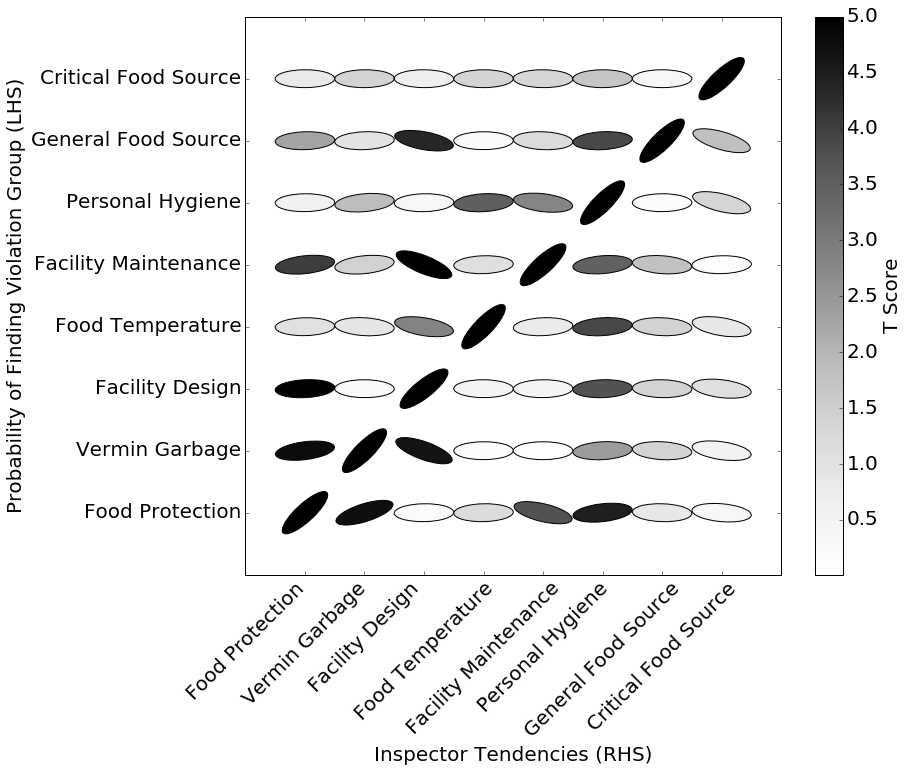
\includegraphics[scale = 0.27]{Task_reg.png}
\end{figure}
\end{frame}

\begin{frame}{5. Are Inspectors Randomly Assigned?}
\begin{itemize}
\item Calculate Inspector Average Scores
\pause
\begin{figure}
    \centering
    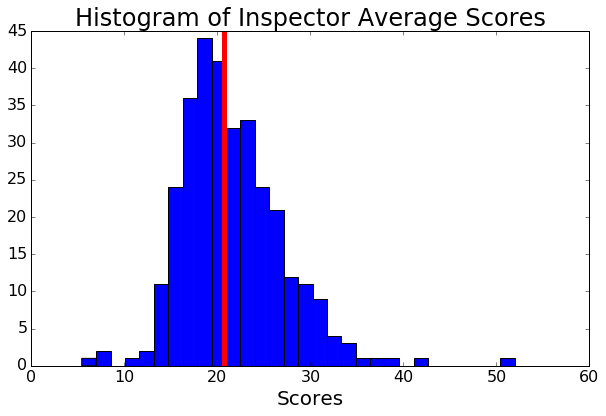
\includegraphics[scale = 0.28]{avg_score_hist.png}
\end{figure}
\pause
\item Split sample into inspections done by inspectors with average scores above and below median average score 
\item Test $H_0$: Distribution of zipcodes, cuisine types, venue types, service types are the same across two samples
\pause
\item Result: fail to reject for all categories (p-values > 0.99). 
\end{itemize}
\end{frame}


\begin{frame}{Sanitation Disclosure Methods Across Cities}
\begin{figure}
    \centering
    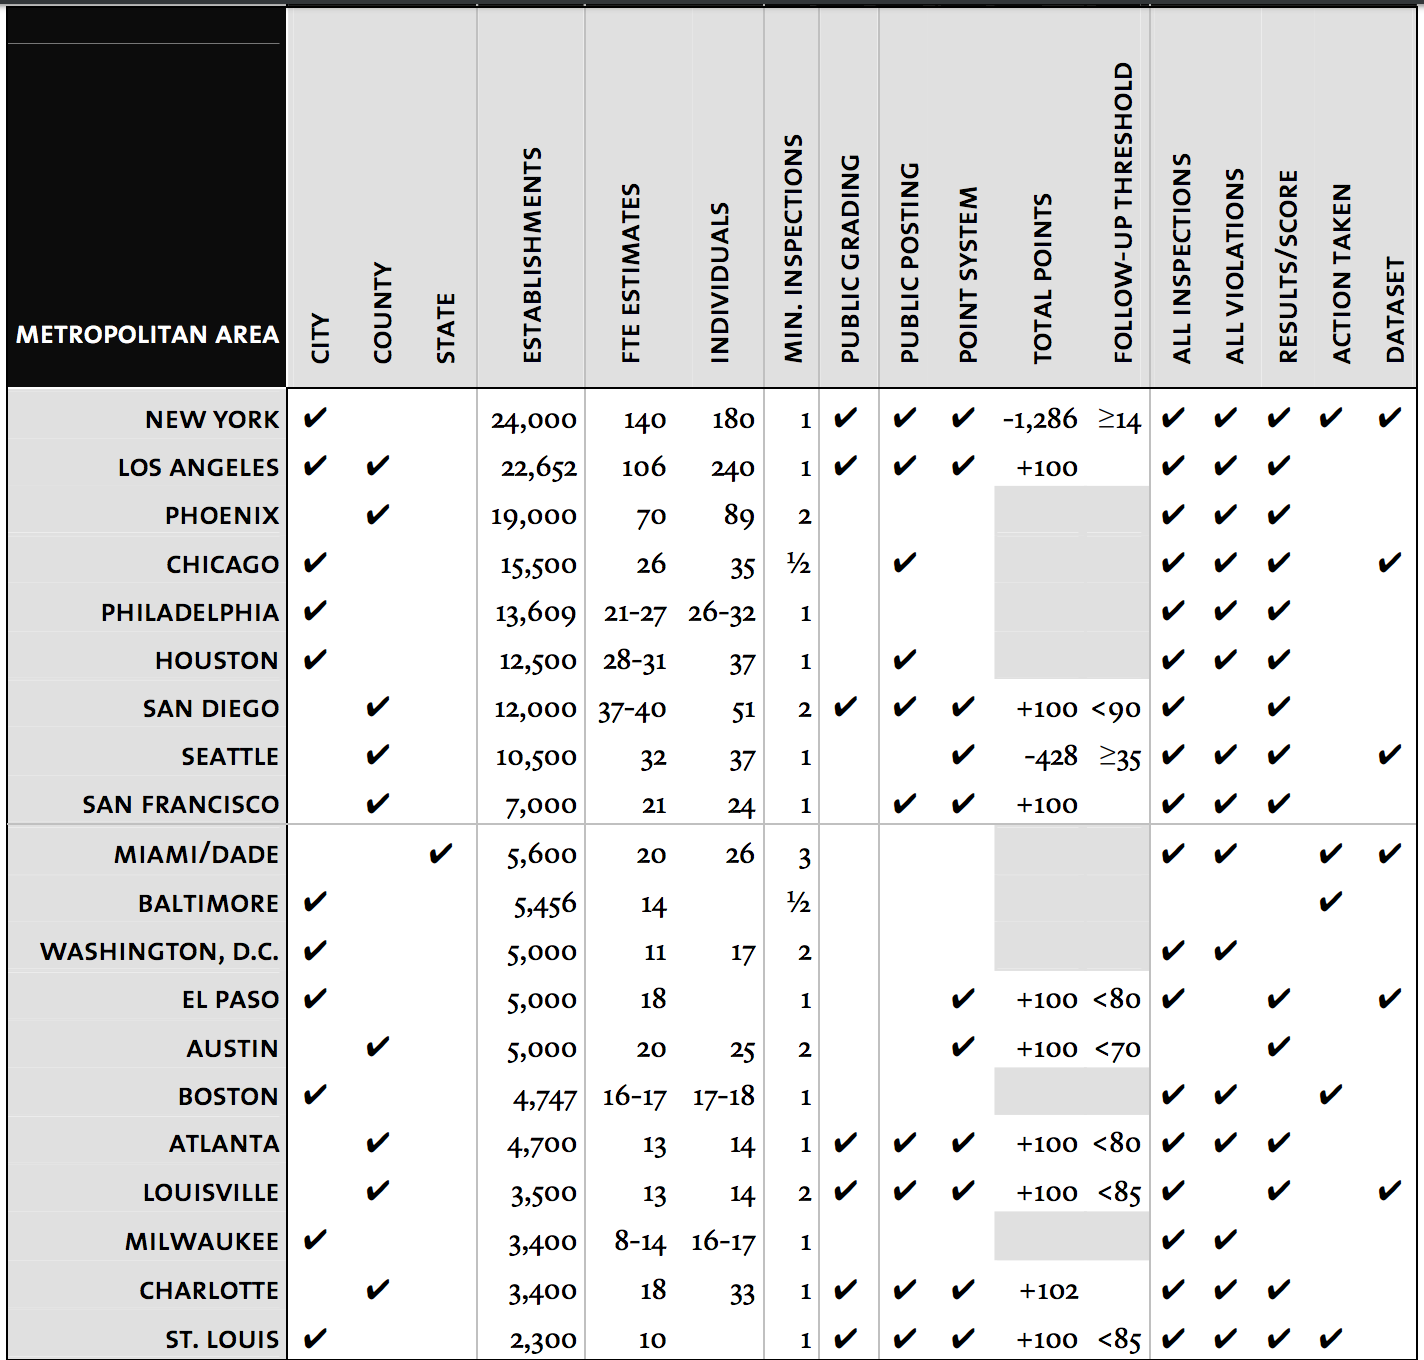
\includegraphics[scale = 0.3]{GradingLandscape.png}
\end{figure}
\footnotesize{Source: Ho (2012)}
\end{frame}


\begin{frame}{Do Inspectors Exercise Similar Discretion Across Different Cuisines?}
    \begin{align*}
        Pr(vio\_sum_i < score_i | vio\_sum \in \mathcal{B}) = \sum_{c \in \mathcal{C}} \beta_c \mathbbm{1}_{\{cuisine_i = c\}} + \varepsilon_i
    \end{align*}
    where $\mathcal{B} = \{12,13,26,27\}$, include time FE. 
\end{frame}

\begin{frame}{Is the Grading System Fair Across Different Cuisines?}
\pause
\begin{itemize}
\item Some opponents of the NYC grading system the current standards does not align with food preparation practices from certain cuisines
\end{itemize}
\pause
\begin{multicols}{2}
\begin{figure}
    \centering
    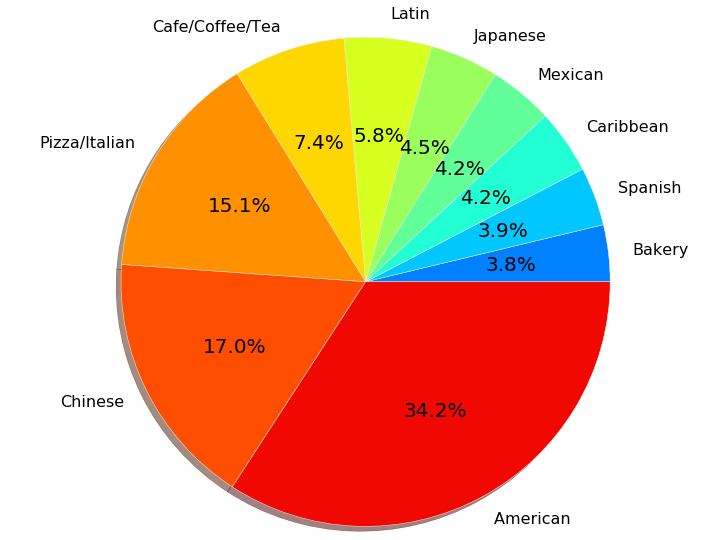
\includegraphics[scale = 0.25]{pie.png}
\end{figure}
\pause
\begin{align*}
    Score_i = \sum_{c \in \mathcal{C}} \beta_c \mathbbm{1}_{\{cuisine_i = c\}} + \varepsilon_i
\end{align*}
\indent $\mathcal{C}$: set of all cuisines
\end{multicols}
\end{frame}

\begin{frame}{Is the Grading System Fair Across Different Cuisines?}
\begin{figure}
    \centering
    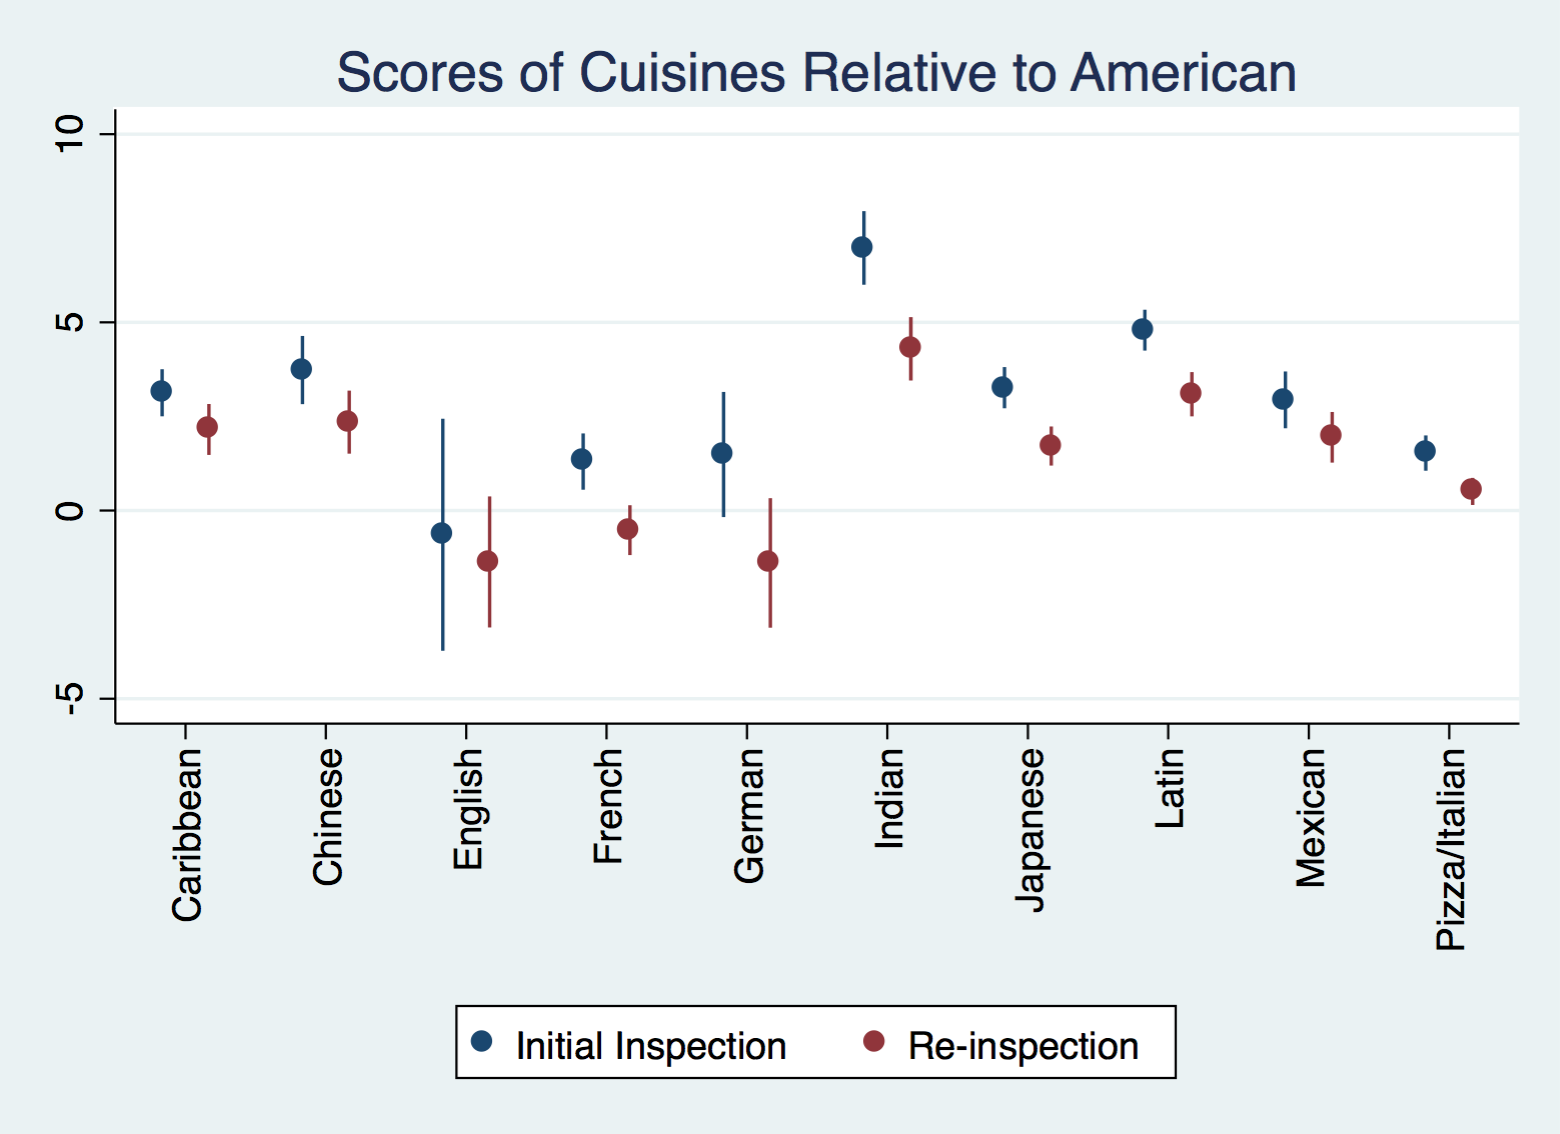
\includegraphics[scale = 0.35]{cuisine_scores.png}
\end{figure}
\end{frame}

\begin{frame}{Which Layout is Best?}
\begin{figure}
    \centering
    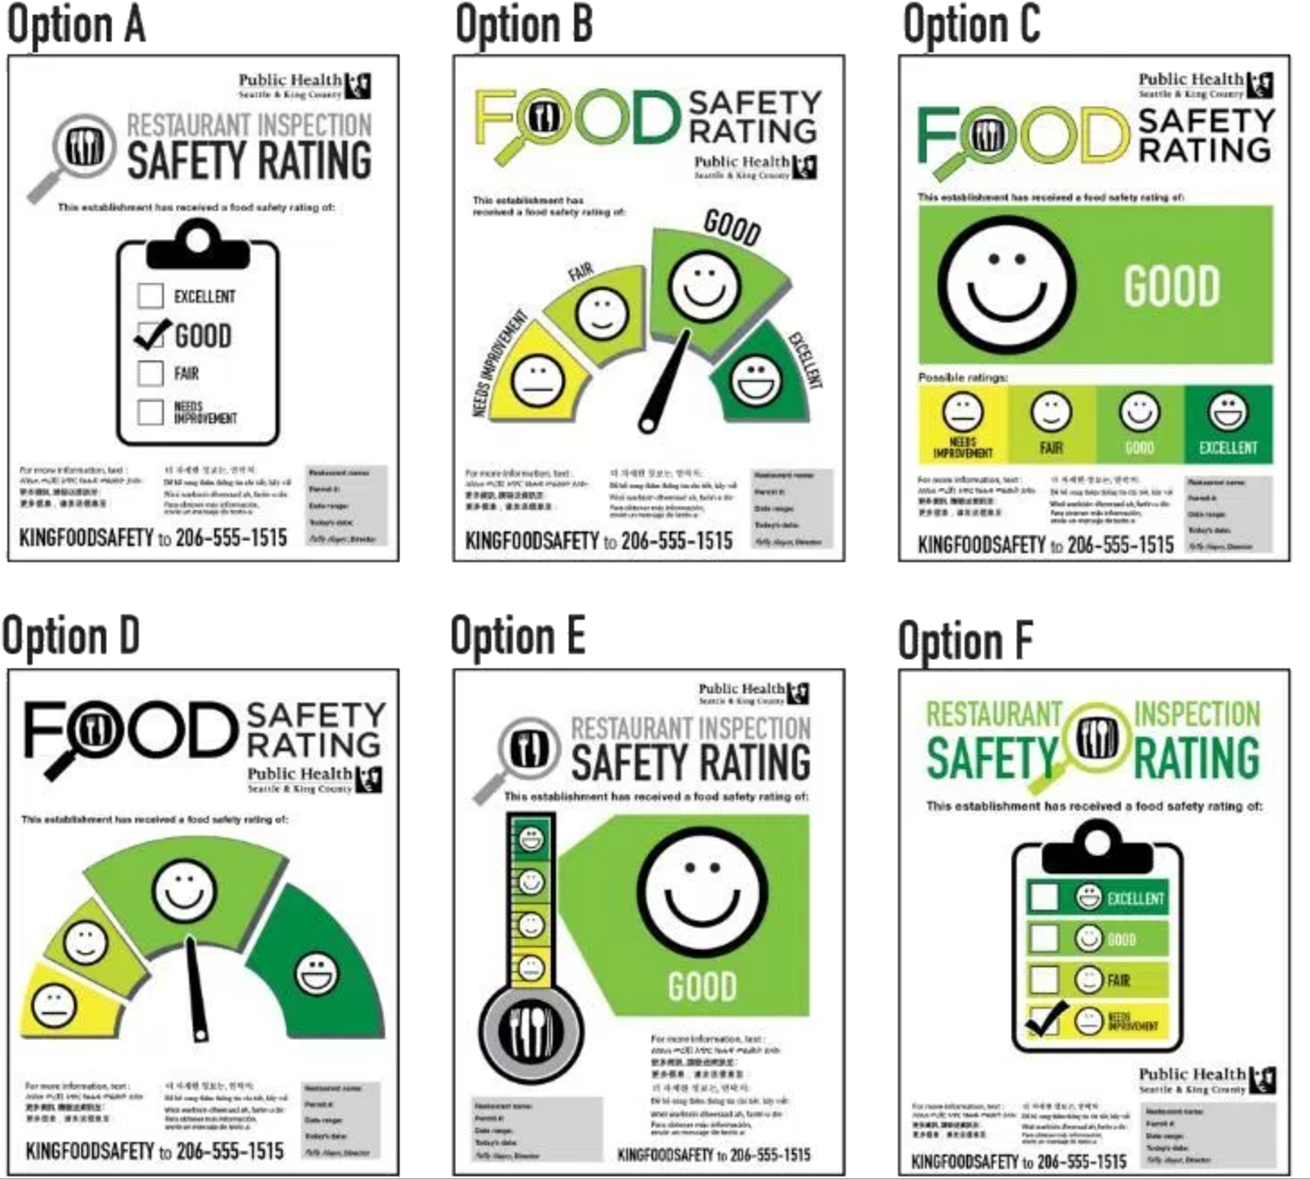
\includegraphics[scale = 0.35]{KingCounty.png}
\end{figure}
\end{frame}